\documentclass{article}
\usepackage{graphicx}
\usepackage[top=2cm, bottom=2cm, left=2cm, right=2cm]{geometry}
%\usepackage{subfig}
\usepackage{subfigure} 
%\usepackage{SIunits}
\usepackage{xspace}
\usepackage{amsmath}
%\usepackage{hepunits}
\usepackage{epstopdf}
\usepackage{tikz}

\DeclareMathSizes{11}{19}{13}{9}

% Alter some LaTeX defaults for better treatment of figures:
    % See p.105 of "TeX Unbound" for suggested values.
    % See pp. 199-200 of Lamport's "LaTeX" book for details.
    %   General parameters, for ALL pages:
    \renewcommand{\topfraction}{0.9}	% max fraction of floats at top
    \renewcommand{\bottomfraction}{0.8}	% max fraction of floats at bottom
    %   Parameters for TEXT pages (not float pages):
    \setcounter{topnumber}{2}
    \setcounter{bottomnumber}{2}
    \setcounter{totalnumber}{4}     % 2 may work better
    \setcounter{dbltopnumber}{2}    % for 2-column pages
    \renewcommand{\dbltopfraction}{0.9}	% fit big float above 2-col. text
    \renewcommand{\textfraction}{0.07}	% allow minimal text w. figs
    %   Parameters for FLOAT pages (not text pages):
    \renewcommand{\floatpagefraction}{0.7}	% require fuller float pages
	% N.B.: floatpagefraction MUST be less than topfraction !!
    \renewcommand{\dblfloatpagefraction}{0.7}	% require fuller float pages

	% remember to use [htp] or [htpb] for placement
	
% Some shorthand
% turn off italics
\newcommand {\etal}{\mbox{et al.}\xspace} %et al. - no preceding comma
\newcommand {\ie}{\mbox{i.e.}\xspace}     %i.e.
\newcommand {\eg}{\mbox{e.g.}\xspace}     %e.g.
\newcommand {\etc}{\mbox{etc.}\xspace}     %etc.
\newcommand {\vs}{\mbox{\sl vs.}\xspace}      %vs.
\newcommand {\mdash}{\ensuremath{\mathrm{-}}} % for use within formulas

% some terms whose definition we may change
\newcommand {\Lone}{Level-1\xspace} % Level-1 or L1 ?
\newcommand {\Ltwo}{Level-2\xspace}
\newcommand {\Lthree}{Level-3\xspace}

% Some software programs (alphabetized)
\providecommand{\ACERMC} {\textsc{AcerMC}\xspace}
\providecommand{\ALPGEN} {{\textsc{alpgen}}\xspace}
\providecommand{\CHARYBDIS} {{\textsc{charybdis}}\xspace}
\providecommand{\CMKIN} {\textsc{cmkin}\xspace}
\providecommand{\CMSIM} {{\textsc{cmsim}}\xspace}
\providecommand{\CMSSW} {{\textsc{cmssw}}\xspace}
\providecommand{\COBRA} {{\textsc{cobra}}\xspace}
\providecommand{\COCOA} {{\textsc{cocoa}}\xspace}
\providecommand{\COMPHEP} {\textsc{CompHEP}\xspace}
\providecommand{\EVTGEN} {{\textsc{evtgen}}\xspace}
\providecommand{\FAMOS} {{\textsc{famos}}\xspace}
\providecommand{\GARCON} {\textsc{garcon}\xspace}
\providecommand{\GARFIELD} {{\textsc{garfield}}\xspace}
\providecommand{\GEANE} {{\textsc{geane}}\xspace}
\providecommand{\GEANTfour} {{\textsc{geant4}}\xspace}
\providecommand{\GEANTthree} {{\textsc{geant3}}\xspace}
\providecommand{\GEANT} {{\textsc{geant}}\xspace}
\providecommand{\HDECAY} {\textsc{hdecay}\xspace}
\providecommand{\HERWIG} {{\textsc{herwig}}\xspace}
\providecommand{\HIGLU} {{\textsc{higlu}}\xspace}
\providecommand{\HIJING} {{\textsc{hijing}}\xspace}
\providecommand{\IGUANA} {\textsc{iguana}\xspace}
\providecommand{\ISAJET} {{\textsc{isajet}}\xspace}
\providecommand{\ISAPYTHIA} {{\textsc{isapythia}}\xspace}
\providecommand{\ISASUGRA} {{\textsc{isasugra}}\xspace}
\providecommand{\ISASUSY} {{\textsc{isasusy}}\xspace}
\providecommand{\ISAWIG} {{\textsc{isawig}}\xspace}
\providecommand{\MADGRAPH} {\textsc{MadGraph}\xspace}
\providecommand{\MCATNLO} {\textsc{mc@nlo}\xspace}
\providecommand{\MCFM} {\textsc{mcfm}\xspace}
\providecommand{\MILLEPEDE} {{\textsc{millepede}}\xspace}
\providecommand{\ORCA} {{\textsc{orca}}\xspace}
\providecommand{\OSCAR} {{\textsc{oscar}}\xspace}
\providecommand{\PHOTOS} {\textsc{photos}\xspace}
\providecommand{\PROSPINO} {\textsc{prospino}\xspace}
\providecommand{\PYTHIA} {{\textsc{pythia}}\xspace}
\providecommand{\SHERPA} {{\textsc{sherpa}}\xspace}
\providecommand{\TAUOLA} {\textsc{tauola}\xspace}
\providecommand{\TOPREX} {\textsc{TopReX}\xspace}
\providecommand{\XDAQ} {{\textsc{xdaq}}\xspace}


%  Experiments
\newcommand {\DZERO}{D\O\xspace}     %etc.


% Measurements and units...

\newcommand{\de}{\ensuremath{^\circ}}
\newcommand{\ten}[1]{\ensuremath{\times \text{10}^\text{#1}}}
%\newcommand{\unit}[1]{\ensuremath{\text{\,#1}}\xspace}
%\newcommand{\mum}{\ensuremath{\,\mu\text{m}}\xspace}
%\newcommand{\micron}{\ensuremath{\,\mu\text{m}}\xspace}
%\newcommand{\cm}{\ensuremath{\,\text{cm}}\xspace}
%\newcommand{\mm}{\ensuremath{\,\text{mm}}\xspace}
%\newcommand{\mus}{\ensuremath{\,\mu\text{s}}\xspace}
\newcommand{\keV}{\ensuremath{\,\text{ke\hspace{-.08em}V}}\xspace}
\newcommand{\MeV}{\ensuremath{\,\text{Me\hspace{-.08em}V}}\xspace}
\newcommand{\GeV}{\ensuremath{\,\text{Ge\hspace{-.08em}V}}\xspace}
\newcommand{\TeV}{\ensuremath{\,\text{Te\hspace{-.08em}V}}\xspace}
%\newcommand{\PeV}{\ensuremath{\,\text{Pe\hspace{-.08em}V}}\xspace}
%\newcommand{\keVc}{\ensuremath{{\,\text{ke\hspace{-.08em}V\hspace{-0.16em}/\hspace{-0.08em}}c}}\xspace}
%\newcommand{\MeVc}{\ensuremath{{\,\text{Me\hspace{-.08em}V\hspace{-0.16em}/\hspace{-0.08em}}c}}\xspace}
%\newcommand{\GeVc}{\ensuremath{{\,\text{Ge\hspace{-.08em}V\hspace{-0.16em}/\hspace{-0.08em}}c}}\xspace}
%\newcommand{\TeVc}{\ensuremath{{\,\text{Te\hspace{-.08em}V\hspace{-0.16em}/\hspace{-0.08em}}c}}\xspace}
%\newcommand{\keVcc}{\ensuremath{{\,\text{ke\hspace{-.08em}V\hspace{-0.16em}/\hspace{-0.08em}}c^\text{2}}}\xspace}
%\newcommand{\MeVcc}{\ensuremath{{\,\text{Me\hspace{-.08em}V\hspace{-0.16em}/\hspace{-0.08em}}c^\text{2}}}\xspace}
%\newcommand{\GeVcc}{\ensuremath{{\,\text{Ge\hspace{-.08em}V\hspace{-0.16em}/\hspace{-0.08em}}c^\text{2}}}\xspace}
%\newcommand{\TeVcc}{\ensuremath{{\,\text{Te\hspace{-.08em}V\hspace{-0.16em}/\hspace{-0.08em}}c^\text{2}}}\xspace}

\newcommand{\pbinv} {\mbox{\ensuremath{\,\text{pb}^\text{$-$1}}}\xspace}
\newcommand{\fbinv} {\mbox{\ensuremath{\,\text{fb}^\text{$-$1}}}\xspace}
\newcommand{\nbinv} {\mbox{\ensuremath{\,\text{nb}^\text{$-$1}}}\xspace}
%\newcommand{\percms}{\ensuremath{\,\text{cm}^\text{$-$2}\,\text{s}^\text{$-$1}}\xspace}
%\newcommand{\lumi}{\ensuremath{\mathcal{L}}\xspace}
%\newcommand{\Lumi}{\ensuremath{\mathcal{L}}\xspace}%both upper and lower
%
% Need a convention here:
\newcommand{\LvLow}  {\ensuremath{\mathcal{L}=\text{10}^\text{32}\,\text{cm}^\text{$-$2}\,\text{s}^\text{$-$1}}\xspace}
\newcommand{\LLow}   {\ensuremath{\mathcal{L}=\text{10}^\text{33}\,\text{cm}^\text{$-$2}\,\text{s}^\text{$-$1}}\xspace}
%\newcommand{\lowlumi}{\ensuremath{\mathcal{L}=\text{2}\times \text{10}^\text{33}\,\text{cm}^\text{$-$2}\,\text{s}^\text{$-$1}}\xspace}
\newcommand{\LMed}   {\ensuremath{\mathcal{L}=\text{2}\times \text{10}^\text{33}\,\text{cm}^\text{$-$2}\,\text{s}^\text{$-$1}}\xspace}
\newcommand{\LHigh}  {\ensuremath{\mathcal{L}=\text{10}^\text{34}\,\text{cm}^\text{$-$2}\,\text{s}^\text{$-$1}}\xspace}
\newcommand{\hilumi} {\ensuremath{\mathcal{L}=\text{10}^\text{34}\,\text{cm}^\text{$-$2}\,\text{s}^\text{$-$1}}\xspace}

% Some usual physics terms

\newcommand{\zp}{\ensuremath{\mathrm{Z}^\prime}\xspace}

% SM (still to be classified)

\newcommand{\kt}{\ensuremath{k_{\mathrm{T}}}\xspace}
\newcommand{\BC}{\ensuremath{{B_{\mathrm{c}}}}\xspace}
\newcommand{\bbarc}{\ensuremath{{\overline{b}c}}\xspace}
\newcommand{\bbbar}{\ensuremath{{b\overline{b}}}\xspace}
\newcommand{\ppbar}{\ensuremath{{p\overline{p}}}\xspace}
\newcommand{\ccbar}{\ensuremath{{c\overline{c}}}\xspace}
\newcommand{\JPsi}{\ensuremath{{J}\hspace{-.08em}/\hspace{-.14em}\psi}\xspace}
\newcommand{\bspsiphi}{\ensuremath{B_s \to \JPsi\, \phi}\xspace}
%\newcommand{\ttbar}{\ensuremath{{t\overline{t}}}\xspace}
\newcommand{\AFB}{\ensuremath{A_\text{FB}}\xspace}
\newcommand{\EE}{\ensuremath{e^+e^-}\xspace}
\newcommand{\MM}{\ensuremath{\mu^+\mu^-}\xspace}
\newcommand{\TT}{\ensuremath{\tau^+\tau^-}\xspace}
\newcommand{\wangle}{\ensuremath{\sin^{2}\theta_{\text{eff}}^\text{lept}(M^2_\mathrm{Z})}\xspace}
\newcommand{\ttbar}{\ensuremath{{t\overline{t}}}\xspace}
\newcommand{\stat}{\ensuremath{\,\text{(stat.)}}\xspace}
\newcommand{\syst}{\ensuremath{\,\text{(syst.)}}\xspace}
% these moved to similar defs
%\newcommand{\Etmiss}{\ensuremath{E_{\mathrm{T}\!{\rm miss}}}}
%\newcommand{\VEtmiss}{\ensuremath{{\vec E}_{\mathrm{T}\!{\rm miss}}}}

%%%  E-gamma definitions
\newcommand{\HGG}{\ensuremath{\mathrm{H}\to\gamma\gamma}}
\newcommand{\gev}{\GeV}
\newcommand{\GAMJET}{\ensuremath{\gamma + \text{jet}}}
\newcommand{\PPTOJETS}{\ensuremath{\mathrm{pp}\to\text{jets}}}
\newcommand{\PPTOGG}{\ensuremath{\mathrm{pp}\to\gamma\gamma}}
\newcommand{\PPTOGAMJET}{\ensuremath{\mathrm{pp}\to\gamma +
\mathrm{jet}
}}
\newcommand{\MH}{\ensuremath{\mathrm{M_{\mathrm{H}}}}}
\newcommand{\RNINE}{\ensuremath{\mathrm{R}_\mathrm{9}}}
\newcommand{\DR}{\ensuremath{\Delta\mathrm{R}}}



% Physics symbols ...

\newcommand{\PT}{\ensuremath{p_{\mathrm{T}}}\xspace}
\newcommand{\qt}{\ensuremath{q_{\mathrm{T}}}\xspace}
\newcommand{\pt}{\ensuremath{p_{\mathrm{T}}}\xspace}
\newcommand{\ET}{\ensuremath{E_{\mathrm{T}}}\xspace}
\newcommand{\HT}{\ensuremath{H_{\mathrm{T}}}\xspace}
\newcommand{\et}{\ensuremath{E_{\mathrm{T}}}\xspace}
\providecommand{\Em}{\ensuremath{E\hspace{-0.6em}/}\xspace}
\providecommand{\Pm}{\ensuremath{p\hspace{-0.5em}/}\xspace}
\providecommand{\PTm}{\ensuremath{{p}_\mathrm{T}\hspace{-1.02em}/}\xspace}
\providecommand{\PTslash}{\ensuremath{{p}_\mathrm{T}\hspace{-1.02em}/}\xspace}
\newcommand{\ETm}{\ensuremath{E_{\mathrm{T}}^{\text{miss}}}\xspace}
%\providecommand{\ETslash}{\ensuremath{E_{\mathrm{T}}\xspace}
\providecommand{\ETslash}{\ensuremath{E_{\mathrm{T}}\hspace{-1.1em}/}\xspace}
%\newcommand{\ETslashi}{\ensuremath{E_{\mathrm{Ti}}\xspace}
\providecommand{\ETslashi}{\ensuremath{E_{\mathrm{Ti}}\hspace{-1.1em}/}\xspace}
\newcommand{\MET}{\ensuremath{E_{\mathrm{T}}^{\text{miss}}}\xspace}
\newcommand{\ETmiss}{\ensuremath{E_{\mathrm{T}}^{\text{miss}}}\xspace}
\newcommand{\VEtmiss}{\ensuremath{{\vec E}_{\mathrm{T}}^{\text{miss}}}\xspace}

% roman face derivative
\providecommand{\dd}[2]{\ensuremath{\frac{\mathrm{d} #1}{\mathrm{d} #2}}}
%%%%%%
% From Albert
%

\newcommand{\ga}{\ensuremath{\gtrsim}}
\newcommand{\la}{\ensuremath{\lesssim}}
%\def\ga{\mathrel{\rlap{\raise.6ex\hbox{$>$}}{\lower.6ex\hbox{$\sim$}}}}
%\def\la{\mathrel{\rlap{\raise.6ex\hbox{$<$}}{\lower.6ex\hbox{$\sim$}}}}

\newcommand{\swsq}{\ensuremath{\sin^2\theta_W}\xspace}
\newcommand{\cwsq}{\ensuremath{\cos^2\theta_W}\xspace}
\newcommand{\tanb}{\ensuremath{\tan\beta}\xspace}
\newcommand{\tanbsq}{\ensuremath{\tan^{2}\beta}\xspace}
\newcommand{\sidb}{\ensuremath{\sin 2\beta}\xspace}
\newcommand{\alpS}{\ensuremath{\alpha_S}\xspace}
\newcommand{\alpt}{\ensuremath{\tilde{\alpha}}\xspace}

\newcommand{\QL}{\ensuremath{Q_L}\xspace}
\newcommand{\sQ}{\ensuremath{\tilde{Q}}\xspace}
\newcommand{\sQL}{\ensuremath{\tilde{Q}_L}\xspace}
\newcommand{\ULC}{\ensuremath{U_L^C}\xspace}
\newcommand{\sUC}{\ensuremath{\tilde{U}^C}\xspace}
\newcommand{\sULC}{\ensuremath{\tilde{U}_L^C}\xspace}
\newcommand{\DLC}{\ensuremath{D_L^C}\xspace}
\newcommand{\sDC}{\ensuremath{\tilde{D}^C}\xspace}
\newcommand{\sDLC}{\ensuremath{\tilde{D}_L^C}\xspace}
\newcommand{\LL}{\ensuremath{L_L}\xspace}
\newcommand{\sL}{\ensuremath{\tilde{L}}\xspace}
\newcommand{\sLL}{\ensuremath{\tilde{L}_L}\xspace}
\newcommand{\ELC}{\ensuremath{E_L^C}\xspace}
\newcommand{\sEC}{\ensuremath{\tilde{E}^C}\xspace}
\newcommand{\sELC}{\ensuremath{\tilde{E}_L^C}\xspace}
\newcommand{\sEL}{\ensuremath{\tilde{E}_L}\xspace}
\newcommand{\sER}{\ensuremath{\tilde{E}_R}\xspace}
\newcommand{\sFer}{\ensuremath{\tilde{f}}\xspace}
\newcommand{\sQua}{\ensuremath{\tilde{q}}\xspace}
\newcommand{\sUp}{\ensuremath{\tilde{u}}\xspace}
\newcommand{\suL}{\ensuremath{\tilde{u}_L}\xspace}
\newcommand{\suR}{\ensuremath{\tilde{u}_R}\xspace}
\newcommand{\sDw}{\ensuremath{\tilde{d}}\xspace}
\newcommand{\sdL}{\ensuremath{\tilde{d}_L}\xspace}
\newcommand{\sdR}{\ensuremath{\tilde{d}_R}\xspace}
\newcommand{\sTop}{\ensuremath{\tilde{t}}\xspace}
\newcommand{\stL}{\ensuremath{\tilde{t}_L}\xspace}
\newcommand{\stR}{\ensuremath{\tilde{t}_R}\xspace}
\newcommand{\stone}{\ensuremath{\tilde{t}_1}\xspace}
\newcommand{\sttwo}{\ensuremath{\tilde{t}_2}\xspace}
\newcommand{\sBot}{\ensuremath{\tilde{b}}\xspace}
\newcommand{\sbL}{\ensuremath{\tilde{b}_L}\xspace}
\newcommand{\sbR}{\ensuremath{\tilde{b}_R}\xspace}
\newcommand{\sbone}{\ensuremath{\tilde{b}_1}\xspace}
\newcommand{\sbtwo}{\ensuremath{\tilde{b}_2}\xspace}
\newcommand{\sLep}{\ensuremath{\tilde{l}}\xspace}
\newcommand{\sLepC}{\ensuremath{\tilde{l}^C}\xspace}
\newcommand{\sEl}{\ensuremath{\tilde{e}}\xspace}
\newcommand{\sElC}{\ensuremath{\tilde{e}^C}\xspace}
\newcommand{\seL}{\ensuremath{\tilde{e}_L}\xspace}
\newcommand{\seR}{\ensuremath{\tilde{e}_R}\xspace}
\newcommand{\snL}{\ensuremath{\tilde{\nu}_L}\xspace}
\newcommand{\sMu}{\ensuremath{\tilde{\mu}}\xspace}
\newcommand{\sNu}{\ensuremath{\tilde{\nu}}\xspace}
\newcommand{\sTau}{\ensuremath{\tilde{\tau}}\xspace}
\newcommand{\Glu}{\ensuremath{g}\xspace}
\newcommand{\sGlu}{\ensuremath{\tilde{g}}\xspace}
\newcommand{\Wpm}{\ensuremath{W^{\pm}}\xspace}
\newcommand{\sWpm}{\ensuremath{\tilde{W}^{\pm}}\xspace}
\newcommand{\Wz}{\ensuremath{W^{0}}\xspace}
\newcommand{\sWz}{\ensuremath{\tilde{W}^{0}}\xspace}
\newcommand{\sWino}{\ensuremath{\tilde{W}}\xspace}
\newcommand{\Bz}{\ensuremath{B^{0}}\xspace}
\newcommand{\sBz}{\ensuremath{\tilde{B}^{0}}\xspace}
\newcommand{\sBino}{\ensuremath{\tilde{B}}\xspace}
\newcommand{\Zz}{\ensuremath{Z^{0}}\xspace}
\newcommand{\sZino}{\ensuremath{\tilde{Z}^{0}}\xspace}
\newcommand{\sGam}{\ensuremath{\tilde{\gamma}}\xspace}
\newcommand{\chiz}{\ensuremath{\tilde{\chi}^{0}}\xspace}
\newcommand{\chip}{\ensuremath{\tilde{\chi}^{+}}\xspace}
\newcommand{\chim}{\ensuremath{\tilde{\chi}^{-}}\xspace}
\newcommand{\chipm}{\ensuremath{\tilde{\chi}^{\pm}}\xspace}
\newcommand{\Hone}{\ensuremath{H_{d}}\xspace}
\newcommand{\sHone}{\ensuremath{\tilde{H}_{d}}\xspace}
\newcommand{\Htwo}{\ensuremath{H_{u}}\xspace}
\newcommand{\sHtwo}{\ensuremath{\tilde{H}_{u}}\xspace}
\newcommand{\sHig}{\ensuremath{\tilde{H}}\xspace}
\newcommand{\sHa}{\ensuremath{\tilde{H}_{a}}\xspace}
\newcommand{\sHb}{\ensuremath{\tilde{H}_{b}}\xspace}
\newcommand{\sHpm}{\ensuremath{\tilde{H}^{\pm}}\xspace}
\newcommand{\hz}{\ensuremath{h^{0}}\xspace}
%\newcommand{\Hz}{\ensuremath{H^{0}}\xspace}
%\newcommand{\Az}{\ensuremath{A^{0}}\xspace}
%\newcommand{\Hpm}{\ensuremath{H^{\pm}}\xspace}
%\newcommand{\sGra}{\ensuremath{\tilde{G}}\xspace}
%\newcommand{\mtil}{\ensuremath{\tilde{m}}\xspace}
%\newcommand{\rpv}{\ensuremath{\rlap{\kern.2em/}R}\xspace}
%\newcommand{\LLE}{\ensuremath{LL\bar{E}}\xspace}
%\newcommand{\LQD}{\ensuremath{LQ\bar{D}}\xspace}
%\newcommand{\UDD}{\ensuremath{\overline{UDD}}\xspace}
%\newcommand{\Lam}{\ensuremath{\lambda}\xspace}
%\newcommand{\Lamp}{\ensuremath{\lambda'}\xspace}
%\newcommand{\Lampp}{\ensuremath{\lambda''}\xspace}
%\newcommand{\spinbd}[2]{\ensuremath{\bar{#1}_{\dot{#2}}}\xspace}
%\newcommand{\MD}{\ensuremath{{M_\mathrm{D}}}\xspace}% ED mass
%\newcommand{\Mpl}{\ensuremath{{M_\mathrm{Pl}}}\xspace}% Planck mass
\newcommand{\Rinv} {\ensuremath{{R}^{-1}}\xspace}
\newcommand{\pb}{\ensuremath{\text{PbWO}_{4}}\xspace}

\begin{document}\setlength{\unitlength}{1mm}
%\begin{verse}
 %      You are writing a Thesis Proporsal in which  you want to answer the following questions:

%why the proposed project is of interest to the HEP community, and perhaps the whole physics community. inevitably involves some theory background.
%What have been done experimentally elsewhere...In my case, the current AN note,CDF etc.
%What  you will do differently to improve the results further beyond the luminocity increase.
 %\end{verse}


\title{Search for Supersymmetry with Gauge-Mediated Breaking in Displaced Photon Events using ECAL Timing and Missing Transverse Energy in \emph{PP} Collisions at $\sqrt{S} = 8$~TeV}
\author{Tambe Ebai Norbert}
\maketitle
\begin{abstract}
Particles with long lifetime also known as long lived particles are predicted to exist in nature by some models beyond the SM. GMSB model is an example of such a model. It
predicts the Neutralino(~$\tilde{\chi}_{1}^{0}$) being the NLSP to decay into a LSP-the gravitino~($\tilde{G}$) and a photon~$(\gamma)$. The photon because of the
neutralino long life time will arrive late at the detector while the weakly interacting gravitino will emerge as an imbalance in the transverse momenta of all the reconstructed
particles in an event. 
In this article, we propose a search for neutralino produced in  $\sqrt{S}=8$~TeV proton-proton collisions through its decay into a photon and a gravitino.
The photon time is measured using the ECAL while the imbalance in transverse momentum also known as $\vec{\ETmiss}$ calculated from transverse momentum measurement using 
the tracker, ECAL and the HCAL of the CMS detector is used to infer the presence of the gravitino.

% We present an analysis to search for long-lived particles decaying into photons in $\sqrt{S}=8$~TeV proton-proton collisions using the CMS detector. We plan on using 
 %the missing transverse energy, \ETmiss and the timing information to search for an excess of events over background prediction. 
%Our analysis involves the decay of neutralino~$(\tilde{\chi}_{1}^{0})$ into a photon~$(\gamma)$ and a weakly interacting ~gravitino $(\tilde{G})$.
\end{abstract}


\section{Introduction}
\paragraph*{}
Supersymmetry~(SUSY) is believed to be a symmetry in nature between bosons~-integer spin and fermions~-half integer spin particles.
It is an extension of the standard model~(SM) predicting the existence of massive neutrally charged particles that can often decay into a photon and a stable
weakly interacting particle. The long life time of these particles implies most of them will travel a few distance from their point of production before
decaying inside the detector. As a result, most of the photons produced through their decay will not emerge from the point of production of these particles
as normal~(SM) photons will but rather
from a secondary position. Such photons will arrive late at the Electromagnetic calorimeter~(ECAL) pointing off the crystal's major axis 
at the arrival point compared to most normal photons originating from the production point.
They are said to be ``Off-Pointing''~(OP) or ``Displaced Photons''~(DP).
Meanwhile the stable weakly interacting particle will travel through the detector undetected. Its presence however can be infered using the imbalance in transverse
momenta calculated from the total transverse momentum of all the reconstructed particles in a event. This imbalance in transverse momenta is also known as the missing
transverse momentum~$\vec{\ETmiss}$.
The presence of a DP and a weakly interacting particle will give a unique topological signal not resulting from known interactions currently described by the SM.
Thus using the ECAL to mearsure the time of arrival of these photons which they are supposed to arrive late because of their displaced vertices and calculating correctly the \ETmiss in each event
might indicate the presence of new physics~(NP).
%Physics scenarios beyond the Standard Model(SM) predict massive, neutrally charged particles decaying into photons. 
%These particles are predicted to have relatively long lifetime. Most of these photons do not originate from the 
%collision point and are refered to as ``Off-Pointing''(OP) or ``Displaced Photons''(DP).
%DP give a unique topological signature which might indicate the presence of New Physics(NP).
%Measuring their time of arrival at the Electromagnetic Calorimeter (ECAL) can be used for their identification. 
%The ECAL has a reliable timing resolution~\cite{TIME}.
%\newline 
%On the other hand, we can only infer (in the transverse direction to the beam line) the presence of particles which do not interact with any section of the detector 
%through calculation of missing transverse energy.
\newline
 This note presents the main features of the search for DP and gravitino using the CMS detector. It is organized as follows: 
In section 1, we give a theoretical motivation of a phenomenological model describing the neutralino production and decay while 
section 2 contains a description of the subdetectors in the CMS detector useful in our search: the tracker, the electromagnetic and hadronic calorimeters. 
A brief analysis strategy is given in section 3, including %we accommodate the definition and performance of 
some important variables we hope will be useful
in separating background from signal and ending with our current work on the analysis. Our conclusion is in section 4 of this article.

\subsection{Theory}
\paragraph*{}
There are lots of published articles explaining the different ways in which Supersymmetry~(SUSY) is spontaneously broken.
A popular understanding of spontaneously broken SUSY is that the Vacuum Expectation Value~(VEV) of an auxiliary field \text{F}
 which is neccessary for maintaining this symmetry~(SUSY) up to the quantum level~(Off-Shell) suddenly becomes non-zero.
However, at our present easily accessible energy scales through accelerators testing models like SM, we do not observe such a symetry between bosons and fermions.
Thus a common speculation is that SUSY breaking cannot occur at energy scales close to SM or supersymmetric extensions of SM 
such as the  Minimal Supersymmetric Standard Model~(MSSM). One of the consequences of such an occurrence  will be the existence of supersymmetric particles
with their masses smaller than those of the already observed SM particles. Since we are yet to observe such particles from current experiments
at the electro-weak energy scale with mass less than 173~GeV ~\cite{ATLAS}, 
it is likely that SUSY breaking if possible must happen at some higher energy scale or early universe period
probably in some set of fields entirely not connected to the fields in the MSSM.
These set of fields are usually refered to as the \emph{``Hidden Sector''} in some SUSY breaking models.
The communication or mediation of SUSY breaking from this high~(thousands or millions of ~TeV) energy scale down to our MSSM energy scales~(few TeV) can be done 
through gravitational, gauge interactions or anomaly in the topology.
SUSY breaking models are developed  based on any 1,2 or all 3 of these interactions depending on certain phenomenology observations to be explained.
\newline
In this article, we focus on Gauge Mediated Supersymmetry Breaking~(GMSB) models  as these are both theoretically and experimentally motivating.




%The breaking of Supersymmetry(SUSY) is not well understood. Where by breaking, we mean, the vacuum is no longer invariant under the symmetry.
% The general assumption is that, the breaking of supersymmetry occurs spontaneously in a set of fields almost entirely not 
%connected to the fields
% in the Minimal Super-symmetric Standard Model(MSSM). However, if the breaking occurs explicitly in the  MSSM, then the superpartners must be \emph{lighter}
% than the corresponding Standard Model(SM) particle. This will be a phenomenological disaster, because we have not yet seen any supersymmetry particle a
%the electro-weak energy scale having a mass less than 173~GeV ~\cite{ATLAS}
%Thus breaking  must occur in some \emph{``Hidden Sector''}, and it is then communicated to the MSSM fields through one of the following 
%mechanisms: gravitational interactions, gauge interactions or an anomaly(a symmetry that occur only at the classical level).
%One of these mechanisms may dominate; however it is possible that all may contribute at once.
%\newline
%The gauge mediated scenario is of prime interest because of its extensive phenomenological features. We mention a few of them in the next section.% as general motivation for 
%gauge mediated SUSY-breaking(GMSB).
\subsubsection{Motivation}
\paragraph*{}
% The first motivation for interest in GMSB models is that 
 A first motivation for GMSB model is that, among many SUSY models build with constraints from cosmology, for example, the constraint that any SUSY model should give rise to an acceptable dark matter density
between $0.1 \leq \Omega_{\chi}\text{h}^{2} \leq 0.3 $ as observed in ~\cite{KOlive}, 
 it predicts that the gravitino is a candidate particle for cold dark matter with its contribution  to this density given as
$\displaystyle{\Omega_{\frac{3}{2}}\text{h}^{2}  = \frac{m_{3/2}}{\text{keV}}\left[\frac{100}{\text{$g_{*}(T_{f})$}}\right]}$ ~\cite{GMSB}. 
$m_{\frac{3}{2}}$ is the mass of the gravitino  and  $g_{*}(T_{f})$ is a function quantifying the effective degrees of freedom of the gravitino at $T_{f}$~( being the 
temperature of the early universe when its contribution remains constant with respect to the rate of expansion of the universe). This degree of freedom is usually between
100 to 200 in SUSY models. \text{h} is known in cosmology as the  Hubble constant given in units of $100$~kmsec$^{-1}$Mpc$^{-1}$.
 %The physics community, no tably the theoretical community, in interested towards 
\newline
 A second motivation for GMSB models comes from comparing theoretical prediction to experimental low energy measurements of the  anomalous magnetic moment of the muon.
Measurements made by the Muon $g_{\mu} - 2$ collaboration in ~\cite{g2ex} compared to SM predictions in ~\cite{g2Theory} suggest that 
$a_{\mu} = \frac{g_{\mu} - 2}{2} $, up to theoretically as well as experimentally understood uncertainties must lie within 
$ -6\times 10^{-10} < a_{\mu} < 58\times 10^{-10} $. This range of uncertainty in the agreement between experiment and SM prediction paves the way for any would-be disagreement 
to be interpreted as the existence of SUSY particles contributing to the SM prediction given in GMSB models as
$\delta a_{\mu}\simeq 15\times10^{-10}(\frac{100GeV}{\tilde{m}})^{2}\tan\beta $.  $\tilde{m}$ is the typical mass scale of weakly interacting SUSY particle and
$\tan{\beta}$ is a free parameter of the theory.
Other low energy measurments  like the branching ratio of the rare decay of B-messons~( in parton level given as  $ b\rightarrow s\gamma$) as found by the CLEO collaboration ~\cite{BSex} to be
within a range  $ 2\times 10^{-4} < $ BR($b\rightarrow s\gamma$) $ < 4.15 \times 10^{-4}$ compared with results from prediction in GMSB suggest the 
existence of SUSY particles contributing to this decay rate.
\newline
Meanwhile, from a theoretical position, GMSB models are  particularly interesting because they make predictions of decay rates and cross sections which do not lead to excesses in
Flavor Changing Neutral Currents~(FCNC) which is yet to be observed experimentally in such large quantities as predicted by other SUSY breaking models
such as constraint MSSM ~(mSUGRA).
They are the closest among all other SUSY breaking models to providing direct understanding to why the Plank energy scale ~($M_{p}=10^{19}$~GeV) is very 
different from the Electro-Weak energy scale~($E_{EWK}\approx 100$~GeV).
 
%Gauge Mediated Supersymmetry-Breaking(GMSB) models provide a solution to the ``Naturalness Problem" otherwise known as the Hierarchy problem.
%It is somehow a technical problem asking why the electroweak energy scale($E_{EWK}\approx 100$~GeV) is so different in magnitude 
%from the Planck energy scale($M_{p}=10^{19}$~GeV)~\cite{SM}. An interesting observation is that most versions of this model have similar phenomenology.
%\newline
%There are contributions to the decay of B-mesons into photons from SUSY particles(sparticles) in GMSB models. %Branchine Ratio(BR); $BR(B \rightarrow \chi_{s}\gamma)$ from
%Measurements of the muon anomalous magnetic moment, $a_{\mu}$, do have sparticle contributions given as
%$\delta a_{\mu}\simeq 15\times10^{-10}(\frac{100GeV}{\tilde{m}})^{2}\tan\beta $ ~\cite{GMSB}, where $\tilde{m}$ is the typical mass scale of weakly interacting SUSY particle.
%Thirdly, GMSB theories present possible scenarios for implementing the strong CP problem. 
%It is also strongly believed that
%Neutral and stable particles like gravitino in the GMSB, could be candidate dark matter particles contributing to the energy density as 
%$\displaystyle{\Omega_{\frac{3}{2}}\text{h}^{2}  = \frac{m_{3/2}}{\text{KeV}}\left[\frac{100}{\text{$g_{*}(T_{f})$}}\right]}$ ~\cite{GMSB}. 
%$T_{f}$ is the freeze  out temperature, and $g_{*}(T_{f})$ is the effective number of degrees of freedom at $T_{f}$ between 100 and 200 in SUSY models.
 %\text{h} is Hubble constant given in units of $100~km~sec^{-1}~Mpc^{-1}$. Indeed, gravitinos depending on their mass could be ``warm'' or ``cold'' dark matter candidates. 
% and in particular we will consider the simplest which we believe is experimentally favourable(meaning we can probe SUSY breaking paramters and so good detecting capabilities for which the neutralino has a long lifetime). 

%\paragraph*{}
%An interesting GMSB scenrio, given as one of the supersymmetry search benchmark points in~\cite{SUSY} 
%is the case in which the lightest neutralino $(\tilde{\chi}_{1}^{0})$ is the Next-to-Lightest Supersymmetric Particle(NLSP). 
%It decays almost exclusively $(>96\%)$  into a photon$(\gamma)$ and a weakly interacting, stable gravitino $(\tilde{G})$  considered to be the Lightest Supersymmetric Particle(LSP)
%($\displaystyle{\tilde{\chi}_{1}^{0} \rightarrow \tilde{G} + \gamma }$). The $(\tilde{G})$ gives rise to \ETmiss by leaving the detector without depositing any energy since it is neutral
%and cannot ionize or interact electromagnetically with other particles in the detector material. According to the choice of parameters, the neutralino lifetime can be non-zero and would
% produce a sample of off pointing photons.
%First, we begin by laying emphasis from a theory point of view our motivation.
\subsection{Phenomenology}
\paragraph*{}
 GMSB models consist of two main sectors. The \emph{observable sector} containing the quarks, leptons and the two Higgs doublets,
 together with their super-symmetric partners (MSSM) and the \emph{hidden sector} which is responsible for SUSY breaking. 
%This secluded sector is usually unspecified because of lack of a standard description, and we will do the same here.
%Rather we will concentrate on the idea that,
\newline 
This breaking must occur in such a way that its effect is felt at the TeV energy scale. Such a SUSY breaking is termed soft breaking which technically means most of the terms in the SUSUY breaking langragian must consist mostly of dimensionful couplings such that
the mass scale cannot exceed the TeV region.
It is these soft terms which provide mass to all of the SUSY partners of the known SM particles.
\newline
Analoguos to the Electroweak symmetry breaking where gauge and Yukawa interactions communicate the Electroweak symmetry breaking to the SM particle states,
in SUSY breaking the original SUSY breaking is also communicated to the ordinary particle supermultiplets. 
However, the only difference is that because of the supertraced theorem, one cannot construct SUSY breaking models where SUSY breaking is communicated to
ordinary supermultiplets through tree level renormalisable couplings as in the Electroweak breaking scenario.
Nevertheless, in the same way as in SM in which the Higgs vacuum expectation value~(VEV) determines the electroweak symmetry breaking so too
in constructing realistic SUSY models we require a chiral superfield $\textsc{X}$ to acquire a VEV and hence determine the scale of SUSY breaking.
$\textsc{X}$ must acquire a VEV along its scaler and auxiliary components as
\begin{equation}
 \langle \textsc{X}\rangle =  \textsc{M} + \theta^{2}\textsc{F}
\end{equation}
 where $\theta$ is a Grassman number.
This analoguos Higgs sector in SM is what is refered to as the hidden or sometimes secluded sector and has no renormalisable tree level couplings to the
``observable sector'' containing ordinary SM and SUSY particles.
\newline
The simplest structure of this secluded sector is the scenario is which the goldstino superfield is $\textsc{X}$ and couples at tree level to 
a ``messenger sector'' formed by some new superfields which transform under a gauge group as a real non-trivial representation.
This tree level coupling generates a supersymmetric mass of the order of $ \textsc{M}$~( one of the main fundamental parameters of any GMSB model) for the 
mass of this messenger field and a mass  squared splittings inside the messenger supermultiplets of the order of $\textsc{F}$~( another fundamental parameter).
$\textsc{M}$ and $\textsc{F}$ are parameters which can  vary from a few TeV to the Plank energy scale.

%In local supersymmetry breaking, the goldstino field  overlaps  with a chiral superfield $\textsc{X}$, which acquire a VEV along the scaler and auxiliary components
%\begin{equation}
% \langle \textsc{X}\rangle =  \textsc{M} + \theta^{2}\textsc{F}
%\end{equation}
%where the parameters $ \textsc{M}$ and $\sqrt{\textsc{F}}$ are fundamental mass scales in the theory and can vary from several tens of TeV to almost  $ 10^{16}$~GeV, the GUT scale.

%\newline 
%The theory also has a \emph{messenger sector}, formed by some new super fields that %transform under the gauge group as a real non-trivial representation 
% couples at tree level with the goldstino superfield \textsc{X}.
%This coupling is responsible for generating a super-symmetric mass of the order of $\textsc{M}$ for the messenger fields and mass-squared splitting inside
% the messenger supermultiplets of the order \textsc{F}. %This sector is also unknown and it is the main source of model dependence.
In a Minimal Supersymmetric Standard Model(MSSM), the messenger sector is described by
$\textsc{N}_{f}$ flavors of chiral superfields $\mathbf{\Phi_{i}}$ and $\mathbf{\bar{\Phi}_{i}}$ $(i=1,\cdots,\textsc{N}_{f})$. 
The interaction  between the chiral messenger superfields $\Phi$ and $\bar{\Phi}$ and the goldstino superfield \textsc{X} is given by the superpotential terms
%transforming as the representation $\boldmath{r} + \boldmath{\bar{r}}$   under the gauge group. 

%To preserve the gauge coupling constant, we require that the messengers form complet GUT multiplets. Such that the presence of messenger fields 
%at an intermediate scale does not modify the value of $\textsc{M}_{GUT}$, but the inverse gauge coupling strength at the unification scale $\alpha^{-1}_{GUT} $ received extra contribution.
%From this extra contribution, we can  have 
%\begin{equation}
 %\displaystyle{\textsc{N} \simeq \frac{150}{\ln\frac{M_{GUT}}{M}}}.
%\end{equation}
 %If \textsc{M} is allowed as low as 100TeV, then \textsc{N} can be at most equal to 5. This upperbound can be relaxed for larger values of \textsc{M}.

\begin{equation}
 \displaystyle{ \textsc{W} \ \ = \ \ \lambda_{ij}\bar{\Phi}_{i}\textsc{X}\Phi_{j} }
\end{equation}
If we replace in eq.(2) the \textsc{X} VEV, see eq.(1), we find that the spinor components of $\Phi$ and $\bar{\Phi}$ form Dirac fermions with masses $\lambda\textsc{M}$, 
while the scalar components have a squared mass matrix  which when diagonalised and solved gives squared masses of the messenger fields as ${\textsc{M}}^{2}\pm \textsc{F}$
~\cite{GMSB},
where the mass scale, $\sqrt{\textsc{F}}$, is the measure of supersymmetry breaking in the messenger sector. 
\newline
The messenger fields couple to the observable sector in a way that unification of couplings is preserved 
 and by gauge invanriance the masses of vector bosons  and fermions is also preserved.
Splitting arises at quantum level because of gauge interactions between fields in the observable sector and messenger fields.
 The main assumption here is, the positivity of the messenger squared mass  which requires  $\text{F} < \text{M}^{2}$. In fact the most realistic case is to
 assume $\text{F} \ll \text{M}^{2}$. 
This assumption makes it possible that in an effective field theory below the messenger scale \textsc{M},
super-symmetry breaking can be treated as a small effect. 
The procedure is as follows: starting from an effective field theory valid for mass scale \textsc{M} 
and integrating out all heavy messenger fields, 
we can solve the renormalization-group(RG) equations in the exact SUSY theory. At the end, we replace \textsc{X} with the VEV,
 to obtain physical mass spectrum for the soft terms to find the mass difference between the SUSY particles and the SM particles is within the TeV energy scale.~\cite{GMSB}.
\newline 
 One very important feature of the gauge-mediated mass spectrum is flavor universality meaning,
the messenger fields interact with all particles with different flavor or different generation in the same way which is a consequence of the symmetry of gauge interactions. 
If we require that gravity-mediated contributions are small, say one per mill of the soft squared masses so as not to break the flavor universality, then
gravity generates soft terms with typical size
 $\displaystyle{\textsc{F}/ \textsc{M}_{\textsc{P}}}$. This gives a rough upper bound on the messenger scale
\begin{equation}
\displaystyle{\textsc{M} \ \ \leq \ \ \frac{1}{10^{\frac{3}{2}}}\frac{\alpha}{4\pi}\textsc{M}_{\textsc{P}}\sim 10^{15}~GeV}
\end{equation}
where $ \displaystyle{ \textsc{M}_{\textsc{P}}  = (8\pi \textsc{G}_{\textsc{N}})^{-1/2} = 2.4 \times 10^{18} GeV }$ is the reduced Planck mass.
However, there are other models which indicate upper bound on messenger scale of $\textsc{M} \leq 10^{13}~GeV$.

\subsubsection{Gravitino as LSP}
Spontaneous super-symmetry breaking produces a physical spectrum containing a massless spin-1/2 fermion called the goldstino.
Coupling the globally super-symmetric theory to gravity produces a locally super-symmetric theory in which the goldstino provides the longitudinal modes of the spin-3/2 
partner of the graviton, the gravitino.
The result of this superhiggs mechanisms is that, the gravitino acquires a super-symmetry-breaking mass which, under the condition of vanishing cosmological constant, is given by
\begin{equation}
 \displaystyle {m_{\frac{3}{2}}} \ \ = \ \ {\displaystyle\frac{F_{0}}{\sqrt{3}\textsc{M}_{\textsc{P}}} }
\end{equation}
$\textsc{F}_{0}$ is the total contribution of the super-symmetry-breaking VEV of the auxiliary fields, normalized such that the vacuum  energy of the globally SUSY theory 
is $\textsc{V}  = \textsc{F}^{2}_{0}$.
$\textsc{F}_{0}$ is not the same as \textsc{F} which appears in the sparticle masses through $\Lambda = \frac{\textsc{F}}{\textsc{M}}$. In fact,  $\textsc{F}_{0} $ is the 
fundamental scale of super-symmetry breaking, \textsc{F} is the scale
of super-symmetry-breaking felt by the messenger particles, i.e. the mass splitting inside their supermultiplets.
We define  the ratio  $\emph{k}\equiv\frac{\textsc{F}}{\textsc{F}_{0}}$  which depends on how super-symmetry breaking is communicated to the messengers. 
If the communication occurs via direct interaction, then this ratio is just given by 
a constant parameter like the parameter $\lambda $ in eq.(2) above. The communication can also occur radiatively in which case \emph{k} is smaller than 1 as oppose to ~1 
for direct interactions.
We rewrite the gravitino mass as
\begin{equation}
 \displaystyle {m_{\frac{3}{2}} \ \ = \ \ \frac{\textsc{F}}{\emph{k}\sqrt{3}\textsc{M}_{\textsc{P}}} \ \ = \ \ \frac{1}{\emph{k}}\left(\frac{\sqrt{\textsc{F}}}{100TeV}\right)^{2} 2.4~eV},
\end{equation}
where the model-dependent coefficient \emph{k} is such that $\displaystyle{\emph{k} < 1}$, and possibly $\displaystyle{\emph{k}\ll 1}$. 
 $m_{\frac{3}{2}}$ is exactly a measure of gravity-mediated effects. It is indeed the solution to the flavor problem in gauge mediation with 
its effect much smaller than gauge-mediated contributions.
This implies, the gravitino is stable and the LSP.
\newline
Assuming conservation of R-parity, (where R-parity is defined as $ \displaystyle{P_{R}=(-1)^{3(B-L) + 2S}}$ with B and L being baryon and lepton numbers respectively, and S is spin)
supersymmetric particles(sparticles) decay in cascade that leads to gravitino.
Which means, single sparticles cannot decay into SM particles alone and superpartners must be produced in pairs from SM particles.
\newline
To compute the decay rates for neutralino, we need to know the interaction Lagrangian at lowest order in the gravitino field.
With $\displaystyle{ \sqrt{\textsc{F}}\ll \textsc{M}_{\textsc{P}}} $, the dominant gravitino interactions come from its spin-1/2 component, 
the interaction Lagrangian can be computed in the limit of global super-symmetry. In the presence of 
spontaneous super-symmetry  breaking, the super current $J^{\mu}_{Q}$ satisfies the equation
\begin{equation}
 \displaystyle { \partial_{\mu}J^{\mu}_{Q} \ \ = \ \ -\textsc{F}_{0}\gamma^{\mu}\partial_{\mu}\tilde{G} },
\end{equation}
This is the goldstino equation of motion. The corresponding interaction Lagrangian is 
\begin{equation}
\displaystyle{ \mathcal{L} \ \  =  \ \ - \frac{1}{\textsc{F}_{0}} J_{Q}^{\mu}\partial_{\mu}\tilde{G} }.
\end{equation}
 The goldstino couples to bilinear, meaning we replace $J^{\mu}_{Q}$ in eq.(7) by its expression for free fields and obtain
\begin{equation}
\displaystyle{\mathcal{L} \ \ = \ \  - \frac{k}{\textsc{F}}\left(\bar{\psi}_{L}\gamma^{\mu}\gamma^{\nu}\partial_{\nu}\phi - \frac{i}{4\sqrt{2}}\bar{\lambda}^{a}\gamma^{\mu}\sigma^{\nu\rho}\mathcal{F}^{a}_{\nu\rho}\right)\partial_{\mu}\tilde{G} + h.c.}
\end{equation}
 where $\phi$ and $\psi$ are the scaler and fermion components of a generic chiral multiplet and $\lambda^{a} $ and $\mathcal{F}^{a}_{\mu\nu} $ are the Majorana spinor 
and gauge field strength belonging to a vector super-multiplet.
 
For on-shell particles, by using the equation of motion, the golstino Lagrangian in eq.(8) can be written as a Yukawa interaction with the chiral superfields and 
magnetic moment-like interaction with gauge particles,
\begin{equation}
\displaystyle{  \mathcal{L} \ \ = \ \ \frac{\emph{k}}{\textsc{F}}\left[\left(m^{2}_{\psi} - m^{2}_{\phi}\right)\bar{\psi}_{L}\phi + \frac{\textsc{M}_{\lambda}}{4\sqrt{2}}\bar{\lambda}^{a}\sigma^{\nu\rho}\mathcal{F}^{a}_{\nu\rho}\right]\tilde{G} + h.c. }
\end{equation}
 Both goldstino interactions are proportional to the mass splitting inside the super-multiplet and inversely proportional to the scale of super-symmetry breaking.
The next-to-lightest super-symmetry particle(NLSP) plays an  important role the phenomenology of gauge mediation. Assuming R-Parity conservation, 
we expect that all sparticles will promptly decay into cascades leading to the NLSP, with the NLSP then decaying into the gravitino via 1/\textsc{F} interactions.
Therefore, the nature of NLSP determines the signatures in collider experiments.
The possibility of NLSP being a neutralino seems interesting because of its dominant B-ino component~(from mass spectra), for moderate M, N and $\Lambda$. In fact the 
SUSY benchmark point SPS 8 in ~\cite{SUSY} uses the following parameters $\Lambda = 100$~TeV, $\textsc{M}_{mes}=200$~TeV,
$\textsc{N}_{mes}=1$, $\tan\beta = 15$, and $\mu >0$. The neutralino decay rate is calculated as
\begin{equation}
 \displaystyle {\Gamma\left(\tilde{\chi}^{0}_{1}\rightarrow\gamma\tilde{G}\right) \ \ =  \ \ \frac{\emph{k}^{2}\kappa_{\gamma}m^{5}_{\tilde{\chi}^{0}_{1}}}{16\pi\textsc{F}^{2}} \ \ = \ \ \emph{k}^{2}\kappa_{\gamma}\left(\frac{m_{\tilde{\chi}^{0}_{1}}}{100GeV}\right)^{5}\left(\frac{100TeV}{\sqrt{\textsc{F}}}\right)^{4} 2\times10^{-3}~eV},
\end{equation}
$\kappa_{\gamma}$ is a constant parameter depending on the components of $ \tilde{\chi}^{0}_{1}$. This is the most dominant decay mode.
To be able to understand this signal at colliders, we need the average distance traveled by the NLSP with mass $\tilde{m}$ and produced with energy E as
\begin{equation}
\mathsf{L}  \ \ = \ \ \displaystyle{\frac{1}{\kappa_{\gamma}}\left(\frac{100GeV}{\tilde{m}}\right)^{5}\left(\frac{\sqrt{\frac{\textsc{F}}{\emph{k}}}}{100TeV}\right)^{4}\sqrt{\frac{E^{2}}{\tilde{m}^{2}}-1}\times 10^{-2}~cm}
\end{equation}
\paragraph*{} 
 Depending on the value of $\sqrt{\frac{\textsc{F}}{\emph{k}}}$, the NLSP can either decay within microscopic distances or decay well outside the solar system.
\newline
If $\sqrt{\frac{\textsc{F}}{\emph{k}}}$ is large(roughly greater than $10^{6}$~GeV), the  NLSP decays outside of the detector and  behaves like a stable particle 
and the neutralino signature resembles those of the ordinary super-symmetric scenarios with stable neutralino.
\newline
For small $\sqrt{\frac{\textsc{F}}{\emph{k}}}$ (typically  $\leq 10^{6}$~GeV) the NLSP promptly decays and the experimental signature is given by events with missing
 transverse energy, imbalance in the final-state momenta and a pair of photons.
\newline
In the intermediate region between the two regions for $\sqrt{\frac{\textsc{F}}{\emph{k}}}$, things become very much interesting. Here the NLSP decay length could be
 measurable as a vertex displacement of the final-state photon.
This is experimentally interesting or favorable, because it allows a better background rejection. It is also theoretically interesting, because the measurement of the
 decay length gives direct information on the value of $\sqrt{\frac{\textsc{F}}{\emph{k}}}$.
This has additional advantage, since other measurements are mainly sensitive only to the mass scale $\displaystyle{ \Lambda = \frac{\textsc{F}}{\textsc{M}}}$ which roughly 
determines the mass spectrum.
In fact on-going analysis is being carried out to measure and set limits on the NLSP decay length.
%\emph{ Now I introduce the Theory site here.}
%\emph{Theoretical Backing of why this is so?}
%\emph{what has been previously done }  
\subsection{Previous Limits}
\paragraph*{}
 Neutralino search at both electron and hadronic colliders have  previously been performed.
A search analysis at LEP,  a lepton-lepton collider, searching for diphoton plus missing energy events resulted to a combined 95\,\% CL limit on the cross section, 
$\sigma\left(\EE\rightarrow\tilde{\chi}_{1}^{0}\tilde{\chi}_{1}^{0}\right)\times BR\left(\displaystyle{\tilde{\chi}_{1}^{0}\rightarrow\gamma\tilde{G}}\right)$
at $\sqrt{S}=172$~GeV of about $\sigma_{\tilde{\chi}_{1}^{0}} < 0.3$~pb for $ m_{\tilde{\chi}_{1}^{0}}  <  70$~$GeV/c^{2}$ and $\sigma_{\tilde{\chi}_{1}^{0}} <  0.15$~pb for 
 $70$~GeV/$c^{2}$ $ <  m_{\tilde{\chi}_{1}^{0}} < 85$~GeV/$c^{2}$ for neutralino with decay length within $0.1 < c\tau < 50$~cm.
 In a fairly parameter independent way, $ m_{\tilde{\chi}_{1}^{0}} <  73$~GeV/$c^{2}$ are excluded as long as  $\tilde{\chi}_{1}^{0}$ decays occur inside the detector ~\cite{LEP}.
\newline
For a hadron collider experiment, CDF and \DZERO, at Tevatron,  searched for diphoton events with large missing energy  during which the measured missing energy distribution 
were found to be in agreement with SM background.
\DZERO set a bound on the cross section $\sigma(\ppbar\rightarrow\gamma\gamma\MET + X)  < 185$~fb at 95\,\% CL 
corresponding to excluding neutralinos lighter than 70~GeV/$c^{2}$ in decay channel $\displaystyle{\tilde{\chi}_{1}^{0}\rightarrow\gamma\tilde{G}}$ with
 decay length $0.1 < c\tau < 100$~cm~\cite{CDF}.
 In run II of Tevetron, CDFII observed no candidate events in a similar diphoton events with  large missing energy in $2.6\pm0.2$ ~$fb^{-1}$ of $\ppbar$
 collisions at$\sqrt{S}=1.96$~TeV. This resulted in a limit of $m_{\tilde{\chi}_{1}^{0}} > 149$~$GeV/c^{2}$ with lifetimes;  $\tau_{\tilde{\chi}_{1}^{0}} \ll 1$~ns 
 completely excluding neutralinos
 with lifetime;  $\tau_{\tilde{\chi}_{1}^{0}} \leq 2$~ns.
Recently, ATLAS did  a similar diphoton search which resulted to a limit of ${\displaystyle \sigma < \left(22-129\right)}$~fb in the 
context of generalised GMSB with a bino-like neutralino~\cite{ATLAS}.
Another group within the CMS collaborators is currently working on a similar analysis~\cite{Rome}.
\newline
From the above results, it indicates that any search for neutralino in the decay channel of a photon and gravitino, 
must be in the region where the neutralino mass is well above 150~GeV/$c^{2}$ with a lifetime 
$\tau_{\tilde{\chi}_{1}^{0}} \geq 2$~ns. The ECAL detector has a radial length of $\approx1.5$~m corresponding to a lifetime of $\approx5$~ns. 
 Thus if one performs a search for slowly moving neutralinos produced at the LHC, it is clear that there is still enough room to improve on these limits.
\section{CMS Detector}
The main feature of the Compact Muon Solenoid (CMS) apparatus is a superconducting solenoid of 6~m internal diameter providing a field of 3.8~T neccessary for good momentun resolution. 
This field  encloses the silicon pixel and strip tracker, the crystal electromagnetic calorimeter (ECAL) and the brass/scintillator hadron calorimeter (HCAL). 
Very long lived particles like muons are measured in gas-ionization detectors embedded in the steel return yoke located at the outermost section of the detector.
It has a simple structure consisting of the barrel and endcap detectors and an extensive forward calorimetry.
The CMS apparatus has an overall length of 22~m, a diameter of 15~m, and weighs 14\,000 tonnes.  
\subsection{ECAL, HCAL and Tracker}
Calorimeters have a unique property of improving relative energy resolution with increasing energy thus making them indispencable  in high energy physics experiments.
In the decay of neutralino, we espect the photon produced to have a very high energy(above 90GeV) and the gravitino which is weakly interacting to emerge as large missing energy.
Therefore it is imperative to describe how the calorimetry system of CMS is designed to ensure that we can detect these photons. We also provide a brief description of
 the tracking system use for calculating missing transverse energy.
 \subsubsection{ECAL}
 The Ecal consists of the Barrel(\textsc{EB}) region occupying a pseudo-rapidity of $\vert \eta \vert< 1.479 $ and two Endcaps (\textsc{EE}) regions covering $1.479 <\vert \eta \vert < 3.0$.
 Sitting right in front of the \textsc{EE}, is a Preshower(\textsc{ES}) detector made of silicon strip sensors interleaved by lead making it a few radiation length thick.
 Its main purpose is to improve in $\gamma/\pi^{0}$ descrimination in the \textsc{EE} regions.
 \paragraph*{}
 The \textsc{EB} and \textsc{EE} combined consist of 75848 lead tungstate (\pb) scintinlating crystals. At the longitudinal end of each crystal is coupled two 
 Avalanche-Photodiodes(APDs) for \textsc{EB} crystals and  Vacuum-Phototriodes(VPTs) for \textsc{EE} crystals for scintilating light collection developed in the crystals.
 VPTs are used for \textsc{EE} crystals because of their better resistance against high radiation.
 This large number of crystals provide an almost $4\pi$ coverage of solid angle which is important for missing energy calculation. 
 \newline 
 \pb  has a radiation length ($X_{0}$) of $\simeq 0.89$~cm. The total longitudinal length of a crystal in  \textsc{EB} is $ 25.8X_{0}$ and $24.7X_{0}$ in \textsc{EE}
 providing enough absorber thickness for most of the energy of the incident very energetic photon or electron to completely lose through a 
 cascade process in the crystal. This energy loss is mainly through radiation of photons(\emph{Bremsstrahlung}) and pair production. The ``amplitude'' or ``probability'' of these processes is 
 proportional to the nuclear charge or number of electrons, \text{Z} of the material. \pb is a high \text{Z} material which makes it a good choice along
 with other properties like fast scintilation time for ECAL calorimetry. Low energy electrons lose their energy through other processes like ionization and excitation. 
 Eventhough \pb is a heavy material, Compton scattering and photoelectric effect is still possible as most of the photons with energy below a few \MeV have 
 their dominant contribution to energy loss from mainly  these processes.
 \newline
 \pb crystals also have a Moliere radius of $2.4$~cm. This ensures that on average about $95$\,\% of the electromagnetic shower energy is contained within the crystal volume therefore
 reducing the transverse spread of the electromagnetic cascade arising from multiple scattering of electrons. It improves on the estimation of the transverse position
 of impact of the incident particle. This  Moliere radius implies \pb is very dense and compact therefore resistant 
 to radiation making it suitable for a high radiation environment like the LHC.
 \newline
 The crystals are  tapered and arranged in a projective goometry pointing $\approx3^{o}$ away from the mean beam collision point. The purpose
 of this is to minimize inter crystal gaps hence preventing photons or part of the photon cluster from going through these gaps undetected.
 This improves the energy calibration and reduces the contribution to the constant term in the Ecal energy resolution and is the dominant
 contribution for high energies and in missing energy calculations. 
 \newline 
 \pb has a fast( 80\,\% of the light emitted within $25$~ns) scintilation process. It peaks in the blue region ($425$~nm) making photo-detection simpler and reliable in a fast
 (bunch crossing frequency of $40$~MHz) timing requirement environment like the LHC.
Although the light-yield for \pb is rather low ($\approx 70$photons/\MeV), the photodiodes have internal gain ( $50$ for APDs and 10 for VPTs) and good quantum efficiency
of $75$\,\% for APDs and $20$\,\% for VPTs of the emission wavelength. This makes it possible that signals 
from incident particles with energies from a few  to high \GeV can be recorded.
\paragraph*{}
 This homogenous design of the ECAL provides it with a performance which is optimal(by design) in its potential to discover a Higgs in the mass region 
 less than $130$\GeV/$c^{2}$ through the decay $\displaystyle{H\rightarrow\gamma\gamma}$. 
 Homogenous design implies reduced noise in the detector  thus better resolution since only a single material type is in use.
ECAL has a current  timing resolution better than 500~ps for large energy deposits(more than 10-20~GeV in the \text{EB})~\cite{TIME} 
and an energy resolution of ${\displaystyle\sigma/E\approx 0.45\,\%}$ for unconverted photons with energies above 100~GeV~\cite{CMSTDR}.
 
%The scintillation time (~25~ns), small radiation length (9 mm), and radiation hardness of PbWO$_4$ are the reasons 
%that this material was chosen for CMS since they minimize the overlapping of signals in space as well as interactions in the 
%adjacent bunch crossings, and they survive in a high radiation environment of the LHC.
%ECAL consists of $75848$ lead tungstate (\pb) scintilating crystals providing a coverage in pseudo-rapidity  of $\vert \eta \vert< 1.479 $ in a barrel
%region (\textsc{EB}) and $1.479 <\vert \eta \vert < 3.0$ in two endcap regions (\textsc{EE}) to cover a large solid angle region, which is important for minimising 
%false missing transverse energy.
%Because of the relatively fast scintillation decay time, we are able to measure the time of the signal very well, and we take advantage of this for our analysis of delayed photon.
%The timing resolution of ECAL Crystals is better than 500~ps for large energy deposits(more than 10-20~GeV in the barrel)~\cite{TIME}.
 %In fact, \pb has a decay time of 25~ns which is comparable with the LHC bunch  crossing interval of 25~ns.
%This extremely fast scintillation process makes it an excellent material in an environment like the LHC.
% \newline
%The signal is generated in the \pb crystals through an electromagnetic showering process.
%This process is caused by electromagnetic interactions between  high energy photons and electrons through a process called
%\emph{Bremsstrahlung} and pair-production. During pair production, the incoming photon, interacts with the atom to produce an electron and positron pair.
%However, in bremsstrahlung, the energetic electron interacts with the nucleus of the atom and is then accelerated
%such that the accelerated electron radiates off a photon continuing as a less
%energetic  electron. The emitted photon can later pair-produce.
%The continuous Bremsstrahlung and pair-production leads to a cascade  production of photons and electrons called the electromagnetic shower.
%It eventually stops when the photons or electrons become less energetic enough to either pair-produce or bremsstrahlung.
%The light produced by the crystals is collected by photo devices which converts this light into photo current and is then transmitted
%eventually to the front end detector. %After every 25ns, through high-speed data link per crystal, all data is  transported out of the ECAL into the counting room.
%\newline
%In front of the \textsc{EE},
%is a single radiation length thick lead material called, the preshower detector. It consist of two planes of silicon sensors interleaved
%with a 9~mm thickness of lead. Its main purpose is to provide $\pi^{0}-\gamma$ separation by distinguishing converted from unconverted photons.%

 %A  unique capability of crystal total absorption calorimetry is its excellent energy resolution. % and hermetic coverage.
%The CMS ECAL utilizes lead tungstate (PbWO$_4$) crystals to achieve an energy resolution of ${\displaystyle\sigma/E\approx 0.45\,\%}$ 
%for unconverted photons with transverse energies above 100~GeV~\cite{CMSTDR}.
% 
% \subsubsection{ECAL}
%  A  unique capability of crystal calorimetry is its excellent energy resolution and hermetic coverage.
% The CMS ECAL has  an energy resolution of ${\displaystyle\sigma/E(GeV)\approx 0.45\,\%}$.
% It consist of nearly $75848$ lead tungstate (\pb) scintilating crystals providing a coverage in pseudo-rapidity  of $\vert \eta \vert< 1.479 $ in a barrel
% region (\textsc{EB}) and $1.479 <\vert \eta \vert < 3.0$ in two endcap regions (\textsc{EE}).
%  %The lead-tungstate crystals provides a fine granularity of $\Delta\eta\times\Delta\phi=0.0175 \times\ 0.0175$ and $\Delta\eta\times\Delta\phi=0.0175 \times\ 0.0175$ to 
% %$\Delta\eta\times\Delta\phi=0.05 \times\ 0.05$ for \textsc{EB} and \textsc{EE} respectively. 
% It  has a radiation length of $X_0=0.89$cm. This allows for much of the energy lost through radiation before eventual ionization.
% The crystals are arranged with a longitudinal length of 25.8\,$X_0$ in the barrel and 24.7\,$X_0$ in the endcaps, 
% such that the scintilation light produced from each crystal is finely collected by photodiodes glued at the end of each crystal.
% Avalanche Photodiodes(APDs) is used for \textsc{EB} and  Vacuum Phototriodes(VPTs) for \textsc{EE}. These photodiodes have high gain and are less affected by
% the high magnetic field. 
% Energy from incoming particles is converted into light through a process called scintillation. 
% The \pb have a unique property in that, in about 25ns, about 80\,\% of all the incomming particle's energy  used to excite the atoms, is released through the scintillation process.
%  In fact, \pb has a decay time of25ns which is comparable with the LHC bunch  crossing interval of 25ns.
% This extremely fast scintillation process makes it an excellent scintilating  material in a fast decision making and high luminosity region like the LHC.
% The electromagnetic showering process is caused by electromagnetic interactions between  high energy photons and elections through a process called
% \emph{Bremsstrahlung} and pair-production. During pair production, the incoming photon, interacts with the atom to produce an electron and positron pair. 
% Where as, in bremsstrahlung, the energetic electron interacts with the nucleus of the atom and is then accelerated 
% such that the accelerated electron radiates off a photon continuing as a less
% energetic  electron. The emitted photon can later pair-produce. 
% The continuous Bremsstrahlung and pair-production leads to a cascade  production of photons and electrons called the electromagnetic shower.
% The process eventually ends when the photons or electrons become less energetic enough to either pair-produce or bremsstrahlung.
% The scintiallated light is collected by the APDs and VPTs which converts this light into photo current and is then transmitted 
% eventually to the front end detector. After every 25ns, through high-speed data link per crystal, all data is  transported out of the ECAL into the counting room.
% \newline
% In front of the \textsc{EE}, 
% is a single radiation length thick lead material called, the preshower detector. It consist of two planes of silicon sensors interleaved 
% with a total of 3$\,X_0$ of lead. Its main purpose is to provide $\pi^{0}-\gamma$ separation by distinguishing converted from unconverted photons.
\subsubsection{HCAL}
Directly behind the ECAL, is the hadronic calorimeter(HCAL).
Unlike the homogenous ECAL, the HCAL is an inhomogenous sampling calorimeter. 
The  hadronic barrel(\text{HB}) and hadronic endcap(\text{HE}) of the HCAL cover a region in pseudo-rapidity of $\vert \eta \vert < 3$. 
The designed consist of plastic scintilating tiles with wavelength shifting fibers sandwiched between layers of brass or steel as absorber giving 
it a repeated interleaved structure  of absorber/dead( steel or brass)  
and active layers of tiles of  plastic scintilating material. The active material
is used mainly for periodically sampling electromagnetic and hadronic components in the hadronic shower 
while steel and brass act as stopping material for energetic incoming hadrons in the shower.
The  absorber material provide fine granularity  of short  nuclear interaction length while tiles of plastic scintilator
separates charged hadrons like protons, pions($\pi^{\pm}$), kaons($k^{\pm}$)  and neutrons from
electromagnetic physics objects like photon and neutral pions contained in the incident hadronic shower. 
This ability to separate different components of a hadronic shower serves as the basis for some particle reconstruction algorithms making the HCAL 
very usefull in the reconstruction of complex physics objects 
like jets which usually consist of hadronic as well as electromagnetic showers.
The HCAL is thus very important in missing energy calculation.
Quartz fibers for Cerenkov light production placed in a steal mix occupy $3 < \vert \eta \vert < 5$.
 % like Particle Flow analysis(\text{PF}).
 \newline
This inhomogenous design gives the HCAL, an energy resolution of ${\displaystyle \Delta E/E \approx 0.5/\sqrt{E(GeV)} }$ above 250~GeV ~\cite{CMSTDR}.
\paragraph*{}
The HCAL calorimeter  is a sampling calorimeter which means it finds the particle's position, energy and arrival time by using the alternating layers of ``absorber''
and fluorescent ``scintilating'' materials which produce a rapid light pulse when  a particle passes through. Some special optic fibres  collect up this light and supply it
to readout boxes where photodetectors amplify the signal. The amount of light in a given region is summed up over many layers of tile along the 
particle's path through the HCAL in depth called a ``tower''. The total amount of light is a measure of the particle's energy and an indicator of its type.
This sampling is used to separate the hadronic  and energetic  electromagnetic  component of the shower which passed through the ECAL unstopped.
\newline
A hadronic shower is formed when an incident hadron undergoes an inelastic collision with the nucleus of the absorber material 
producing secondary hadrons which as they go through successive layers of
absorber material interact inelastically with other nuclei to produce further hadrons etc. 
The  hadronic cascade loses about 30\,\% of incident hadron energy through nuclear excitation of the nuclei of atoms of the  absorber material.
\newline
The HB calorimeter is an assembly of two half barrels each composed of 18 identical
$20^{o}$ wedges in $\phi$. The wedge is made of flat brass alloy absorber plate parallel to beam axis with the innermost and outermost layers made up of
stainless steal interleaved by plastic scintillator tiles.
The first active layer is situated directly behind the ECAL in order to actively sample low energy showering particles from the support material between the ECAL 
and HCAL. Each scintillator tile has a size of $\Delta\eta\times\Delta\phi=0.087 \times\ 0.087$ 
and is instrumented with a single wave length shifting fiber(WLS) for better collection of light. The summed optical signals or light are converted into fast electronic
signals by photosensors called  hybrid photodiode(HPD).
%The optical signal from the HCAL towers is detected with a pixelated
\newline
In the foward region in $\eta$ is the forward calorimeter (HF) made up of steel absorbers embedded in radiation hard quartz fibers running parallel to the 
beam axis and providing a fast collection of Cerenkov light. The signal results from Cerenkov light emitted in the quartz 
fibres embedded in the steel matrix in response to charged particles.
The Cerenkov calorimeter have long and short fibers which are positioned alternatively separated by 5~mm with readouts for better 
sampling of the different shower components.
The goal of this hardware design is to give better compensation for different shower components in the hadronic shower.
The HF section enables the HCAL to pick up myriad of particles coming out of the collision region  at very shallow angles relative to the beam direction.
%In fact the steel and brass alloy sandwiched with active tile of scintillator provide a great stopping power for highly energetic events as well as providing fast readout.
\newline
These different sections of the HCAL in $\eta-\phi$ plane give it a unique capability to measure multi-jet events revealing the fine structure of jets.
Decaying particles may produced new particles that do not leave any record  of their presence in any part of the CMS detector.
To spot such particles, the above HCAL sections give it an almost ``hemetic'' coverage making sure it captures  to the extend possible every particle emerging from
collisions.  In this way, if we observe a particle in one side of the detector but not in the other, with imbalance of momentum and energy in the direction
``transverse'' to the beam  direction, we can deduce that we are producing ``invincible''     particles. 
This is the primary idea in missing transverse energy calculation  established as signal for very weakly interacting particles like neutrino and hopefully gravitino.
Generally speaking, in the region $\vert \eta \vert< 1.74$, the HCAL cells have widths of 0.087 in pseudorapidity($\eta$) and 0.087\,rad in azimuth ($\phi$).
In the $(\eta,\phi)$ plane, and for $\vert \eta \vert < 1.48$, 
the HCAL cells map on to $5 \times 5$ ECAL crystals arrays to form calorimeter towers projecting radially outwards from close 
to the nominal interaction point. At larger values of $\vert \eta \vert$, the size of the towers increases and the matching ECAL arrays contain fewer crystals. 
Within each tower, the energy deposits in ECAL and HCAL cells are summed to define the calorimeter tower energies subsequently used to provide the energy
 and direction of hadronic jets. 
% \newline
% All these information is fed into the PF algorithm for particle reconstruction.
 \subsubsection{Tracker}
 Unlike calorimeters, the tracker is basically a magnetic spectrometer where the momentum resolution is linearly  proportional to the particle's momentum 
 in a given  magnetic field.
 This means very low momentum particles have better momentum resolution than their high momentum counterparts.
 The momentum of a charged particle is inversely proportional to the curvature of its trajectory in the magnetic field. 
 By reconstructing the trajectory of the particle as it moves in the tracker; through ``hits'' made at various positions,
 we are able to deduce its curvature and hence determine its momentum.
 High momentum particles are less curved by the magnetic field than low momentum particles.
Thus, the tracker  is expected to have a very good momentum resolution for low momentum particles. The strong magnetic field and high granularity of the 
CMS silicon tracker allows promptly produced charged particles with $\PT = 100GeV/c$ to be reconstructed with a resolution in the transverse momentum \PT  of
 about $\sim 1.5\,\%$.
 The tracker and calorimeter combine to provide good energy resolutioin for low as well as high momentum particles respectively.
\paragraph*{} 
At the LHC design luminocity of $10^{34}~cm^{-2}s^{-1}$ there will be on average $1000$ particles from roughly $23$ overlapping proton-proton interactions traversing
the tracker for each bunch crossing every $25$~ns. A detector technology featuring high granularity and fast response is required such that the trajectories can be identified
reliably and attributed  to the correct bunch crossing.
It is for this reason that the CMS tracker opted for silicon technology. Since silicon sensors are highly suited to receive many particles in a small space 
due to  their fast response  and spatial resolution.
The tracker is tasked along with the ECAL and  muon chambers to identify electrons and muons. Tracking information is also heavily used in the High Level
Trigger (HLT) system of the CMS to reduce the event rate from the LHC bunch crossing rate of $40~MHz$ to about $100~Hz$ which can be permanently stored.
One of the most important goals of the tracker is to minimize the effects on the tracking performance of electron bremsstrahlung and hadronic interactions. For this,
the tracker has a track isolation criteria for identifying photons and electrons from electromagnetic clusters. This criteria is applied to suppress
$\gamma-\pi^{o}(jet)$ and $\pi^{o}-\pi^{o}(jet-jet)$ backgrounds to a level significantly below the irriducible $\gamma-\gamma $ background.
\newline
The CMS tracker achieves this performance by using silicon pixel and  strip trackers. It has about 1440 pixel and 15148 strip detector modules.
The pixel tracker has 3 layers positioned at
radii between 4.4~cm and 10.2~cm while the silicon strip tracker has 10 layers surrounding the pixel detector in the barrel and extending out ward to  a radius of 1.1~m.
Each system is completed by endcaps which consist of 2 disks in the pixel detector and 3 plus 9 disks in the  strip tracker on each side of the barrel extending
the acceptance of the tracker to a pseudorapidity of $\vert\eta\vert < 2.5$. The pixel detector also covers a pseudorapidity  of $ -2.5 < \eta < 2.5$ matching the acceptance of the
 central tracker. It is closest to the beam line directly surrounding the interaction vertex and has
pixels of size $\approx 100 \times 150~\mu m^{2}$ covering a total area of $\approx 1~m^{2}$. The main function of the pixel detector is to provide  precise tracking points
in the $ r-\phi$ and Z responsible for small impact parameter resolution of about $\sim 15~\mu m$  ~\cite{CMSTDR},which is important for
good secondary vertex  reconstruction and position resolution. This is crucial in the identification of  displaced vertex physics objects with life-time of 
about $\tau \approx 10^{-12}~s$. They include particles such as
$B^{0,{\pm}}$, $D^{0,{\pm}}$, $\tau^{\pm}$, which may travel a distinguishable distance (c$\tau$ $\approx 100~\mu$m.) 
before decaying into particles with tracks like electrons and muons. 
In addition, it is also important for forming seed tracks for outer track reconstruction and high level triggering.
\newline
 %The tracker consists of the Silicon Strip Tracker(SST) and Pixel Tracker.
 %Its volume consists of a first layer of pixels followed by strips extending to ~$110$~cm with a total length of 540~cm. 
 %Ecah pixel has a size $\approx 100 \times 150~\mu m^{2}$ providing good vertex and position resolution.
 %Close to the interaction vertex, in the barrel region are 3 layers of hybrid pixel detectors at a radii 4.4, 7.3, and 10.2~cm.
 The silicon strip detector covers the radii region $ 20$~cm$ < r < 110$~cm.
 The over 15,000 silicon modules occupy an active area of $200~m^{2}$ providing a coverage in pseudorapidity up to
 $\vert\eta\vert < 2.5 $. It is also known as the outer tracker and consist of almost 9.6 million silicon strips providing a 
 spatial resolution measured to be about $10~\mu$m for $r-\phi$ measurement and about
$20~\mu$m for Z measurment necessary for particle trajectory reconstruction.
At the intermediate radii ($ 20$~cm$ < r < 55$~cm), where the particle flux is reduced, it is instrumented with silicon micro strip in the barrel detector
with a typical cell size of
$10~cm \times 80~cm$ in $ r-\phi $ and Z plane. The silicon modules here have sensors of thickness about $320~\mu m$,
while for radial distances; $ 55$~cm$ < r < 110$~cm, the strip detector uses longer strips. The strip electric noise scales linearly with its length. Thus in order
to maintain a good signal to noise ratio well above 10, the CMS uses thicker silicon sensors of about $500~\mu m$ which has correspondingly higher signal.
Overal the Strip detector is made of 4 subdetectors. The Inner Barrel (TIB) consists of 4 cylindrical layers while the outer barrel (TOB) has 6 cylindrical layers.
Two endcap detectors(TEC) in the positive and negative side of the Z cordinate consist of 9 carbon fiber disks with petal structure providing support for the modules.
Signals from  modules of both strip and pixel dectors are amplified by 4 to 6 Analogue Pipeline Voltage(APV25) read out chips mounted on the front-end hybrid(FE-hybrid).
The hybrid provide key information such as temperature of the chips and timing information in order to match the recorded ``hits'' with collision.
 
%Measuring the track of charge particles in the tracker provide enough information to calculate it's momentum.
%The inner tracker measures charged particles within the $\vert\eta\vert < 2.4$ pseudo-rapidity range.% It is located in the 3.8T field of the superconducting solenoid. 
%It provides and impact parameter resolution of $\sim 15~\mu m$ and a $\PT$ resolutions of about $1.5\,\% $ for 100~GeV/c particles ~\cite{CMSTDR}
%\newline
% A detailed description of CMS  detector can be found elsewhere ~\cite{JINST}.
\section{Analysis Strategy}
 Neutralino decay would manifest itself as a topological signature where a very energetic photon originates from a vertex displaced from the LHC beam line.
 This displaced point can range from a few milimeters within the ECAL volume to astronomical distances out side the detector. Infact, the decay length
 of neutralino as seen from equation (11) is of the order of :
\begin{equation}
 \mathsf{L}  \ \ \sim \ \ \displaystyle{\frac{\textsc{F}^{2}} {{\tilde{m}}^{5}}}
\end{equation}
 
Therefore, depending on the value of \textsc{F} and the mass of neutralino$ (\tilde{m})$, its decay can be an instantaneous (prompt), non-prompt as well as 
delayed.
This analysis focuses on the search from non-prompt to delayed neutralino decay. As a result, we expect the CMS detector to be most sensitive
 to neutralino decay within the ECAL volume.
 \paragraph*{}
 Neutralino production at the LHC is of primarily two sources.  In the first scenario, neutralino emerges as an end product from some weakly conserving R-parity decay of a
 higher mass SUSY particle. This type of production mechanism is refered to as GMSB.
 Secondly, neutralino can also be directly produced from parton-parton interactions like gluon-gluon fusion or gluon-quark or quark-quark interaction.
\newline
The decay kinematics of neutralino into $\gamma$ and $\tilde{G}$ for each production mechanism will be  unique.
In this analysis we use as benchmark for understanding its kinematics the GMSB-produced neutralino
(We explore other neutralino production mechanisms).
Assuming the nuetralino is produced with very little momentum ( momentum sligthly bigger than its mass) 
such that it is a slowly moving particle and that it decays entirely within the ECAL volume,
our signature candidate for its presence will be events with one or two displaced vertices within the CMS tracker volume 
and photons with high transverse momentum (\PT) and large missing transverse energy (\ETmiss). We believe that these high \PT photons, because of the supposed 
large decay length of the neutralino,  will arrive late at
the ECAL and since SM does not predict any high mass (mass $ > 200~GeV/c^{2}$) and long lifetime ($ \tau > 2~ns$) particles, this is definitely a background free
search with our main background from misreconstructed photons and decays in flight.
With this kind of background, we expect that simple cuts to reduce this background can include:
\begin{enumerate}
 \item Cut on the decay length ( using ECAL Timing).
 \item Cut on the \PT of the photon and its tracker quality( if any).
 \item Cut on the missing transverse energy (\ETmiss).
 \item Other topological cuts relating to how isolated the photon might be as well as the total number of associated jets in the event.
\end{enumerate}
To be precised, the cuts we intend to apply for each event are the following:
On photons, we will expect an isolated photon with a $\PT > 90~GeV/c$ in the pseudorapidity region of $\vert \eta \vert < 2.5$ while on the gravitino,
we use a $\ETmiss > 30~GeV/c^{2}$ to reject SM background missing transverse energy sources as well as detector inefficiency and require the \ETmiss calculation to be within
the pseudorapidity  of the tracker range  $\vert \eta \vert < 2.5$ and across all other subdetectors. Most importantly, we expect events with  $\vert$ ECAL TIME $\vert > 2~ns$ to reduce mostly SM background.



%The %begining phases of our analysis will be to address the following issues:
%\begin{enumerate}
%\item Understand the CMS detector.%using measurement of standard model physics processes.
%item Quantify relevant systematics in detector performance in measuring variables of interest.
%\item Signal sensitivity studies and background rejection efficiency measurement using variables in 2.
%\end{enumerate}

\subsection{Luminosity and Data Selection}
Physics processes beyond the standard model have very small 
cross section. Therefore, measuring an observable of BSM process provides an extra challeng but at the same time an excellent opportunity because these processes have not
been well studied.
%Luminosity is the main factor to every search especially searches for NP since these processes usually have very small cross section.
 We discuss in the following sections; the various factors important to our analysis.
\subsubsection{Luminosity}
 Luminosity expresses the rate at which a certain interaction will occur during proton-proton collisions. It is proportional to the number of particles colliding
and inversely proportional to the transverse size of the bunches at collision. Interaction in CMS is defined to be inelastic 
proton-proton collisions leading to significant energy deposition in the main parts of the detector.
The luminosity depends on the number of properties. For two gaussian distribution proton beams colliding head on, the luminosity dependence can be summarized in the following equation:
\begin{equation}
 {\displaystyle \mathcal{L} \ \ = \ \  \frac{N_{1}N_{2}N_{b}}{4\pi\sigma_{x}\sigma_{y}}f_{\text{rev}} }
\end{equation}

where $\text{N}_{1}$ and $\text{N}_{2}$ are the number of protons in bunch 1 and 2 respectively and $\text{N}_{b}$ is the total number of bunches. $\text{f}_{\text{rev}}$ is the 
revolution frequency of each bunch.
The important factor here is the spread in the bunches in the transverse direction, denoted here as $\sigma_{x}$ and $\sigma_{y}$ 
during collision which depends on the design of the collider.
 The LHC has been designed to run at instantaneous luminosity between
 $ 10^{28}cm^{-2}s^{-1}$ and $10^{34}cm^{-2}s^{-1}$ at a bunch crossing rate of $40.08$~MHz. 
An orbit of the machine comprises of $3564$ bunches with about $10^{11}$ protons per bunch, of which $2835$  have real collisions when running at designed luminosities. 
\newline
The typical cross section for a given physics process is related to the  instantaneous luminosity through:
\begin{equation}
{\displaystyle\textsc{R} \ \ =  \ \ \sigma\times \mathcal{L} } %\ \ ;  \ \  \displaystyle{\textsc{L} \ \ = \ \ \int L_{inst}\mathrm{d}t}
\end{equation}
where \textsc{R} is the observed rate for a physics process with cross section $\sigma$ and $\mathcal{L}$ is the instantaneous luminosity.
The number of events observed from a given physics process is therefore given by \textsc{R}.
The CMS recorded total integrated luminosity of $\displaystyle{\textsc{L}=5.20fb^{-1}}$~\cite{cmsdata}. This is a reasonable amount of 
data for us to begin expecting the presence of
physics process with theoretical cross section within the picobarn and the femtobarn range.
%\newline
% The event rate \textsc{R} can be calculated as :
%\begin{equation}
 %\displaystyle{\textsc{R}  \ \ = \ \ \frac{1}{\tau}\frac{\textsc{N(1-f)}}{\epsilon}\kappa_{pu}\kappa_{dead}}
%\end{equation}
%where \textsc{N} is the number of slected events, $\epsilon$ is the efficiency, $\tau$ is a $5$mins of time interval, \textsc{f}, $\kappa_{pu}$ and $\kappa_{dead}$ are correction factors.
%The interations are defined to be inelastic proton-proton collisions leading to a significant energy depositions int the main parts of the CMS detector.
%The LHC is designed to be running at luminosity range of $ 10^{28}cm^{-2}s^{-1}$ to $10^{34}cm^{-2}s^{-1}$ and probably beyond, and the bunch crossing rate of $40.08$MHz. 
%An orbit of the machine comprises of $3564$ bunches, of which $2835$  have real collisions when running at designed luminosities. 
%By the end of 2010, the first year of LHC operation, proton beams reached a new energy region of  $3.5TeV$ with a peak in instantaneous luminosity of
% $2 \times10^{32}cm^{-2}s^{-1}$ in \emph{pp} collisions. CMS experiment accumulated $43pb^{-1}$ of \emph{pp} data with a efficiency of $92\,\%$.~\cite{cmsdata}.

%\newline
%Supposed we have a certain interaction  with cross section of $\sigma = 80$mb, 
%at a designed instantaneous luminosity of $ 10^{34}cm^{-2}s^{-1}$ with an effective bunch crossing rate of $\textsc{f}_{BX}=\frac{2835}{3564}\times 40.08$MHZ, 
%we have the number of interations per bunch of $\displaystyle{\mu = \frac{\sigma\textsc{L}_{inst}}{\textsc{f}_{BX}}\simeq 25 }$.
%In the minimal model of GMSB(SPS 8 benchmark point) as in ~\cite{SUSY}, the cross section from theoretical calculations and upper limits set by other searches~\cite{ATLAS}, gives
%$\displaystyle{\sigma(pp\rightarrow\tilde{\chi}_{1}^{0} + hadron) < (27-91)}$fb,with same designed luminosity of $10^{34}cm^{-2}s^{-1}$ an 
%perfomance efficiency per-event $\displaystyle{\epsilon=0.9295}$ and per-event fake fraction $\displaystyle{\textsc{f}=0.0064}$, average deadtime $\displaystyle{\kappa_{dt}=1.0033}$
% and Pile-Up correction, $\displaystyle{\kappa_{pu}=1.030}$; using euation 1 and 2, we get a rate of $7-25\,\%$ of BSM events every 5mins in the coming years when the LHC reaches the goal of using  real time measurment to determine the average luminosity with 1\,\% statistical accuracy in 0.1s.

\begin{figure}
\centering
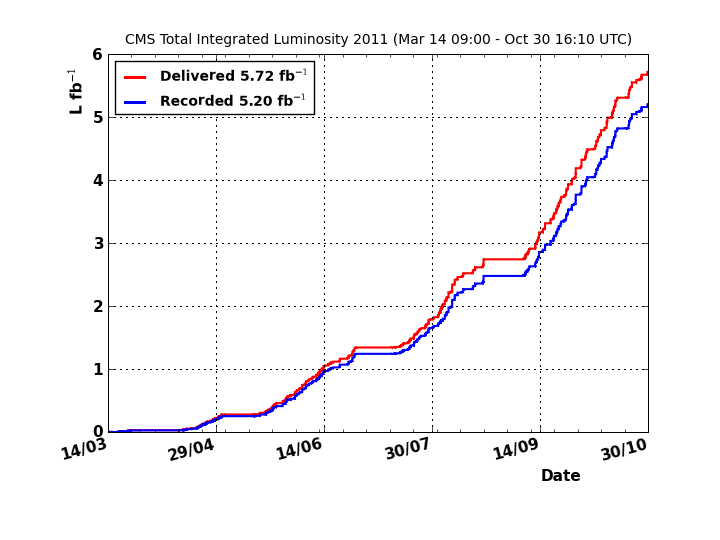
\includegraphics[width=12cm,height=7cm]{/home/tensr/Dropbox/PHD_Thesis_HEP/PhDDeg/totallumivstime-2011.png}
\caption{Total Integrated Luminosity vs Time delivered to (red), and recorded by CMS (blue) during stable beams for pp running at 7 TeV center-of-mass energy.}
\end{figure}
%\subsubsection{CMS Data}
%The data analyzed in this analysis corresponds to an  integrated luminosity of $1721 +/- 77 pb^{-1}$, collected and reconstructed using \emph{$\CMSSW_4_2_8$}. Only luminosity-sections certified as GOOD int the official good run file were used and the datasets analysed correspond to:
%\boldmath{$173.3$pb^{-1}:}/Photon/Run2011A_May10ReReco-v1/AOD
%\boldmath{$553.2$pb^{-1}:}/Photon/Run2011A_PromptReco-v4/AOD
%\boldmath{$670.3$pb^{-1}:}/Photon/Run2011A_05Aug2011-v1/AOD
%\boldmath{$324.7$pb^{-1}:}/Photon/Run2011A_PromptReco-v6/AOD
%\boldmath JSON:Cert_$160404-177515_7$TeVPromptReco-Collisions11_JSON.txt
%\subsubsection{Triggers}
\subsubsection{Data Selection}
Data taking begins with the first level(L1) of the CMS trigger system, 
composed of custom hardware processors. Information from the calorimeter and muon system is used to select the most interesting events.
 The High Level Trigger(HLT) further decreases the event rate from around 100~KHz to 300~Hz, before data storage. 
This is very important as only very interesting physics events are stored for further event selection and there is no space or computer time to keep all the data.
Event selection begins with triggering an interest event during data taking process.
The advantage is that, processing time during analysis is reduced.%, event selection can be done online, as well as offline
%without filling up the storage system with events of lesser interest and to reduce data processing time.
%\subsubsection*{L1 Trigger}
\subsubsection*{On-line Data Selection}
 %The first level(L1) of the CMS trigger system is composed of custom hardware processors for fast decision making. 
%It uses information from the calorimeters and muon detectors to select, in less than $1~\mu$s, the most interesting events.
 The calorimeter trigger works on primitives from two sub-detectors: the electromagnetic calorimeter(to build electron and photon candidates) 
and the hadron calorimeter(which triggers jets.)
Its main goal is to provide a list of the most energetic candidates from different classes, e.g \emph{4e$\gamma$ ,4$\mu$}, 4jets or \textsc{MET}(Missing Transverse Energy). 
The L1 trigger reduces the event rate from \text{40~MHz} to \text{100~KHz}.
In figure 2, we give an example of the performance of an Level 1 ECAL electron trigger, which selects electrons with a threshold of 15~GeV.
 The efficiency is almost one after the threshold.
%\subsubsection*{HLT Trigger}
%\subsubsection*{ Off-line Data Selection}
\paragraph*{}
The High Level Trigger (HLT) code runs on large group of computers further decreases the event rate from around \text{100~KHz} to around \text{300~Hz} 
before data storage by analyzing a full event. It further subdivides the data into data streams with respect to physics. 
%It takes about \textsc{40 $\mu$s} for HLT calculation of one event. %The full and detailed reconstruction of a proton-proton event takes about 2s.
%  An important role of the trigger system is a proper assignment of events to the bunch crossing it originated from.
%  Therefore, data have to be synchronized with the LHC clock by taking into account different sources of delays, such as geometrical delays,
% the time for signal propagation or electronics jitter. %All CMS sub-detectors had performed the synchronization procedure during the start-up of the LHC. 
The data selection requirement normally includes the following:  for a example, with a candidate photon, the selection criteria might include
a high \pt isolated photon(to remove Jets faking photons), with  \pt  above a certain 
threshold(to remove events arising from soft collisions), within a given geometrical region of the calorimeter, usually the \textsc{EB} where  energy resolution is best.
Event selection sometimes require events originating from a given number of interaction vertices and with a given number of Jets associated with them.
This kind of primitive selection also defines the off-line selection.
\newline
Event reconstruction uses a Particle-Flow(PF) algorithm. It consists reconstructing and identifying each  particle with an 
optimized combination of all sub-detector information. The energy of a photon is directly obtained from the ECAL measurement, corrected for zero-suppression effects.
The energy of neutral hadrons is obtained from the corresponding calibrated ECAL and HCAL energy. 
Figure 3 is an example of an HLT Photon trigger, selecting diphoton objects with a minimum transverse momentum of 32~GeV and 26~GeV.
 The efficiency reaches one beyond the 32~GeV threshold.
%% The primary tiggers used for our search is $\mathsf{Photon75-CaloIdVL-IsoL}(runs 160410-165120$) and $ \mathsf{Photon90-CaloIdVL-IsoL}$(runs 165121-173692), where both are seeded using $\mathsf{L1-SingleEG20}$. These triggers have an on line requirement of 
%% %\sigma_{i\etai\eta} < 0.024,
%% %\frac{ECAL Iso}{\et(\gamma)} < 0.2,
%% %\frac{HCAL Iso}{\et(\gamma)} < 0.2, and H/E < 0.15.
%% All off line selection cuts are therefore chosen to be tighter than the HLT selection. We see from Figure~1 that Photon90-CaloIdVL-IsoL becomes 100\,\% efficient with an off line cut of $\pt(\gamma) > 100GeV$.
\begin{figure}[ht]
\begin{minipage}[b]{0.5\linewidth}
\centering
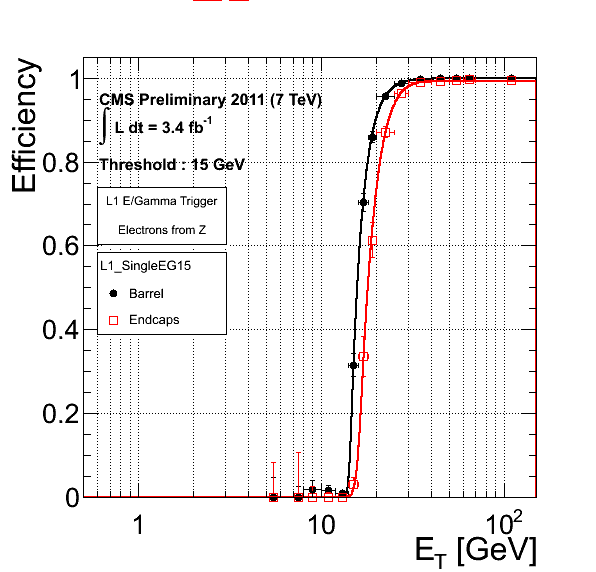
\includegraphics[width=9cm,height=6.1cm,scale=1]{/home/tensr/Dropbox/PHD_Thesis_HEP/PhDDeg/L1ECALElectronTrigger.png}
\caption{Efficiency of Level 1 ECAL Electron Trigger.}
\label{fig:figure1}
\end{minipage}
\hspace{0.5cm}
\begin{minipage}[b]{0.5\linewidth}
\centering
\includegraphics[width=9cm,height=6cm,scale=1]{/home/tensr/tambeebainorbert/Documents/Michaels_Upper_Limit_GMSB.png}%HLTPhotonTrigger.png}
\caption{Efficiency for diphoton HLT Trigger.}
\label{fig:figure2}
\end{minipage}
\end{figure}

\subsection{Missing Transverse Energy(\ETmiss) and Ecal Time Reconstruction}
\paragraph*{} 
In a large signal parameter space, the $\tilde{\chi}_{1}^{0}$  has a non-neglible lifetime($\tau_{\tilde{\chi}_{1}^{0}}$). The decay into
a delayed photon and a neutral gravitino prompts the use of Calorimeter timing and the missing transverse energy(MET) or \MET as background discriminating variables.
The photon time is considered as the ``cluster time'' or in rare cases ``the supercluster time'' where a cluster is a collection of crystals and a super cluster is 
a collection of basic clusters. If the photon energy is spread on many clusters, then it is considered to be a super cluster and the time is calculated using the time of 
impact of the seed cluster (highest energy cluster) in the super cluster.
\subsubsection{ECAL Time Reconstruction}
 %Event Time is defined as time of arrival of each event assumed to be traveling with the speed of light to the front of the ECAL crystals. Since 
\paragraph*{}
Photons travel with the speed of light. Their time of travel from collision point to calorimeter crystals is taken as reference for any other physics object.
From a detector point of view, each photon is seen as a cluster of energy hits on crystals. Therefore, a logical way to define the photon arrival time, is
to find the average of the time measured by each crystal as:
\begin{equation} 
{\displaystyle T_{\gamma} \ \ = \ \ \sum_{i}^{N_{xtal}}\frac{T_{RECO,i}}{N_{xtal}}}
\end{equation}
where  ${\displaystyle i=1,\cdots,N_{xtal}} $ and $ N_{xtal}$ is the number of crystals in the cluster.
 %$ \langle t_{i} \rangle$ is calculated from
where $T_{RECO}$ is the reconstructed time such that avearging over number of events ${\displaystyle \langle T_{RECO} \rangle \approx 0}$.
By definition, ${\displaystyle T_{RECO,i} = T_{RAW,i} + Constant }$.
The constant consist of channel-to-channel inter calibration  and any global phase shift. 
Finding new constants such that on average, ${\displaystyle \langle T_{RECO} \rangle \approx \langle T_{RAW}} \rangle \approx 0$ is called timing calibration. %This is were a lot of timing calibration studies is heavily done.
We obtain $T_{RAW}$ from the reconstructed time $T_{MAX}$. In the following paragraph, we briefly describe the process of obtaining $T_{MAX}$ from the reconstructed hits.
\paragraph*{}
The signal develops when an energetic hit impinge on the crystal. The crystal, through a process of scintillation, convert the energy of the hit into light  which propagate 
through the crystal as an electromagnetic shower to the end of the crystal where it is collected by photo detectors.%(APDs and VPTs for \textsc{EB} and \textsc{EE} respectively). 
The front end electronics amplify and shape the signal from the photo detectors. 
The pulse shape is defined  by the analog part of the front end electronics. For each given channel(crystal), all particles result in the same pulse shape to a very 
good approximation. The pulse is digitized at $40$~MHz by a voltage-sampling analog-to-digital converter on the front end, 
producing discrete samples of the amplitude as illustrated in Figure 4. 
Figure~4(a) shows the typical measured signal pulse in the ECAL after amplification(solid line).
The amplitude of the pulse, \emph{A}, is shown as a function of \emph{$T-T_{MAX}$}. \emph{T} is the time of ADC sample and \emph{$T_{MAX}$}
 is defined as the time when the pulse reaches its maximum value \emph{$A_{MAX}$}.
These samples are stored in a buffer until a Level-1 trigger is received, prompting the transmission of ten consecutive samples to the off-detector electronics for insertion into 
the CMS data stream.
\newline
We define the ECAL time reconstruction as the measurement of \emph{$T_{MAX}$} using the ten available samples of the pulse amplitude. Similarly, ECAL energy reconstruction is defined 
as the determination of the true pulse amplitude, \emph{$A_{MAX}$} ~\cite{RECOAMPLI}.
For each channel, the values of the pulse samples depend on three factors: The value of \emph{$A_{MAX}$}; the relative position of \emph{$T_{MAX}$} between time samples, which will
 be referred to as a ``\emph{$T_{MAX}$} phase'', and the pulse shape itself.
\newline
A very good alternative often used to represent the pulse shape as \emph{A(T)}, is the ratio variable, defined as 
\emph{$\displaystyle{R(T)=\frac{A(T)}{A(T+25ns)}}$}. This has advantage that any systematic errors cancel out.
 Figure~4(b) shows the measured pulse shape using variables \emph{$T-T_{MAX}$ vs R(T)}.
This pulse representation, \emph{T(R)}, is independent of \emph{$A_{MAX}$} (albeit not so true with very low and very high amplitude hits). 
It can  be described very well with a simple polynomial parametrization \emph{T(R)} as seen in Figure~1(b).
A pair of consecutive samples give a direct measurement of the ratio \emph{$\displaystyle{R_{i}=\frac{A_{i}}{A_{i+1}}}$}  
and thus a measurement  for each sample of \emph{$\displaystyle{T_{MAX,i}=T_{i}-T(R_{i})}$}.  
 The uncertainty on each time measurement for each sample, $\sigma_{i}$, is given as a product of the
 derivative of the \emph{T(R)} function and the uncertainty on the value \emph{$R_{i}$},  where $i$ is the $i^{th}$ ratio.
 Ratios with large derivative of \emph{T(R)} and $\emph{A} \approx 0$ are not used, since this is quite closed to the pedestal value.
 This uncertainty in \emph{$R_{i}$}  has three independent contributions which are added in quadrature. The first one is due to noise fluctuations, $\sigma_{n}$, in each sample.
 The second contribution is due to the uncertainty in the estimation of pedestal value
which is subtracted from the measured amplitude in each sample. The last contribution is due to truncation during 12-bit digitization.
\paragraph*{}
Typically, there are four or five ratios available per pulse. The reconstructed time of the hit and its errors are determined using the formula for the weighted average,
assuming that the ratios are uncorrelated:
\begin{equation}
\displaystyle{ \mathsf{ T_{MAX}} \ \ = \ \ \frac{\sum\frac{T_{MAX,i}}{\sigma^2_{i}}}{\sum\frac{1}{\sigma^2_{i}}} }
\end{equation} ;
\begin{equation}
 \displaystyle{ \mathsf{ \frac{1}{\sigma^2_{T}}} \ \ = \ \ \sum\frac{1}{\sigma^2_{i}} } .
\end{equation}

This formula despite its success in medium energy hits, performs poorly with very low ($<2$~GeV) and very high energy($>100$~GeV) hits.
 We are currently working on improving this. Nevertheless, the good thing about this method is that it is less affected by the ``\emph{$T_{MAX}$} phase'' 
than the normal represenation method of figure 1(a).  
Using this algorithm, the time resolution is shown to be less than 400-500~ps~\cite{TIME} for energy deposits larger than 10-20~GeV in the barrel. 
\newline
To be able to evaluate this performance, consider a decay path length of 10~cm for a long-lived particle. 
The ECAL time measurement would equate around 334~ps. This is considerable not very far from a typical in-time measurement for an in-time photon.
 Indeed for the most energetic ECAL crystal with energy $10~GeV < E < 100$~GeV, within the barrel region 
($\vert\eta\vert < 1.479$), the time resolution is about $400-500$~ps, we can still argue that the ECAL time is a 
very powerful variable for identifying displaced photons.
%\paragraph*{}
% Time of flight varies across the ECAL by a few nanoseconds and there are different intrinsic delays among the channels. Therefore a crystal-to-crystal synchronization 
%of the ECAL must be performed. Particles originating from the CMS interaction region(IP) would create a signal with the same average \emph{$T_{MAX}$} in a given ECAL channel.
% This is because proton-proton collisions are synchronized  with the LHC Clock and the time of flight of a relativistic particle from the IP to a given channel does not change. 
%This indicates that we get a better amplitude reconstruction if the ECAL energy deposits of all ECAL channels have the same ``\emph{$T_{MAX}$ Phase}'' within 1~ns.
 %The ECAL front end electronics allows adjustment of the ``\emph{$T_{MAX}$ Phase}'' for groups of $5\times5$ channels in steps of 1.04~ns. We determine the values of these 
%adjustment through a process called Hardware synchronization.~\cite{ECALTDR}. Using physics collision events we can also improve on the value of the ``\emph{$T_{MAX}$ Phase}''
% that corresponds to particles coming from the IP for each ECAL Channel whose accuracy must be better than the typical timing resolution. These corrections are called software 
%synchronization.
%Overall the uncertainty in the determination of the synchronization coefficients , which is the quadratic sum of the statistical and systematic uncertainties is about 300-600~ps 
%~\cite{TIME} which can be drastically improved upon in the coming years. % as we record more data and understand the ECAL better.

\begin{figure}
\centering
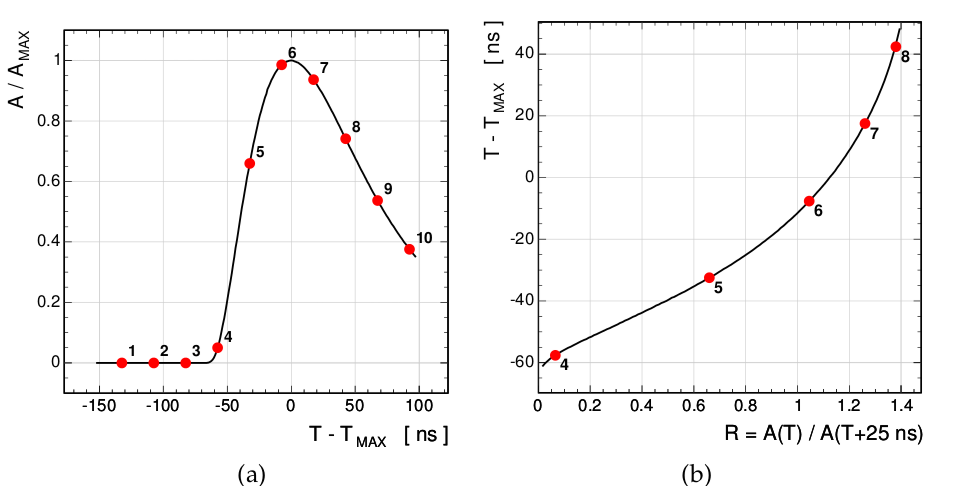
\includegraphics[width=13cm]{/home/tensr/Dropbox/PHD_Thesis_HEP/PhDDeg/TimingPicture.png}
\caption{Left: Typical measured ECAL pulse shape. The \emph{x-axis} represents the distance between the position of the \textsc{ADC} sample~(T) from the expected maximum 
of the pulse shape \emph{$(T_{MAX})$} while the \emph{y-axis} shows the amplitude in each sample normalized to the maximum. 
 Right: \emph{$T-T_{MAX}$} as a function of the value of the measured ratio of the amplitude in two consecutive samples
 (\textsc{R}). The solid line is the average pulse shape as measured with an synchronous beam of electrons. The dots indicate ten discrete samples of the pulse, 
corresponding to a single event.}
\end{figure}

%- So what is \emph{$ECAL_{TIME}$} as used in the analysis? How is it related to \emph{$T_{MAX}$}?
\subsubsection{\ETmiss}
\paragraph*{}
Missing energy is the apparent signal of neutrinos or some weakly interacting stable particles in a detector. Modern detectors at hadron colliders are designed to provide
close to $4\pi$ coverage in solid angle with calorimetry. The CMS detector provides this hermicity with the ECAL and HCAL to calculate missing energy.
\newline
In a hadron collider like the LHC, it is quite challanging to know with very good approximation; along the longitudinal direction of the beam pipe, 
the total energy of the colliding partons making up the protons. 
As a result, energetic particles produced in the direction of the beam pipe makes it almost impossible to directly
measure the energy imbalance (missing energy) parallel to the beam direction. 
On the other hand, since the colliding partons are travelling with very high 
forward momentum or momentum parallel to the beam line, it is
logical to assume that on the plane transverse to the beam pipe just before impact, their total momentum on this plane is zero. Knowing that the initial transverse momentum is zero,
the final( after impact) transverse momentum can be measured to a good approximation such that the transverse energy imbalance defined as the magnitude of the total
transverse momentum imbalance measured is good enough to help establish a physics signature involving one or more non-interacting particles. 
\newline
With this assumption that the total transverse momentum of the partons in the proton just before collision is very minimal or zero and 
using conservation of transverse momentum (momentum transverse to the beam pipe),
the total sum of the transverse momentum of all the particles produced after collision must also equal zero.
After carefully measuring the transverse momentum for all the particles  which deposited energy in the calorimeter and left tracks in the tracker as they interacted with 
the detector, the transverse momentum imbalance  is considered as the momentum or energy carried away by the weakly-interacting particles produced.
This transverse momentum imbalance is also called the missing transverse momentum vector \textbf{\ETmiss}. \ETmiss is considered as the physics signature for energetic
neutrinos or other weakly interacting stable particles.
The discovery of  the \text{W} in the decay ${\displaystyle\textsc{W} \rightarrow \ell\nu}$ used \ETmiss. The electron is observed as an energy deposit in the ECAL
with a track in the tracker while the neutrino is identified by the \ETmiss calculated event-by-event.
Missing transverse energy corrections arising from detector inefficiency is extracted in the low \ETmiss region by measuring the transverse mass of \text{W} 
and \text{Z} to be applied in the measurement of high \ETmiss where the measurement is not very reliable. The purpose of this is to improve the mearsurement of high \ETmiss.
\newline
The belief that other new particles produced at the hadron collider will express themselves through \ETmiss has led to deligent studies of \ETmiss in terms of identifying
other sources of \ETmiss which may not be real and could result from the many inherent detector inefficiency.
\paragraph*{}
Reconstruction of missing transverse energy vector; $\vec{\ETmiss}$ involves ECAL and HCAL cells combined to form  calorimeter towers with the $\eta$ and $\varphi$ of the tower segmentation defined to match
the granularity of the hadron calorimeter or HCAL geometry. $\vec{\ETmiss}$ is calculated by summing individual calorimeter towers having energy $E_{n}$ and
pseudorapidity $\eta_{n}$ and azimuthal angle $\varphi_{n}$ as:

\begin{equation}
 \displaystyle{ \vec{\ETmiss} \ \ = \ \ -\sum_{n}\left(\frac{E_{n}\cos\varphi_{n}}{\cosh\eta_{n}} \hat{x}  +  \frac{E_{n}\sin \varphi_{n}}{\cosh\eta_{n}}\hat{y}\right) \ \ = \ \ E^{Miss}_{x} \hat{x} + E^{Miss}_{y} \hat{y} }
\end{equation}


Physics objects like muons which deposit very small amount of energy in the calorimeter(about $4$~\GeV) are taken into account and their calorimeter energy deposit replaced
with their reconstructed track \pt.
\newline
Other possible sources of miss measured \ETmiss include: Noise in the HCAL, cosmic muons traversing the detector, beam halo, cracks in the detector as well as misidentification
of physics objects in the reconstruction of the total transverse energy.
Despite all these challenges in \ETmiss calculation, better and smarter algorithms have been developed which take into consideration all these sources of fake \ETmiss.
A very good algorithm which is very reliable is the (PF) \MET algorithm which is a common tool for calculating \ETmiss. It uses charged track corrections 
where \pt measurement from the tracker replaces their  corresponding ECAL energy. Removal of fake sources of \MET like noise from HCAL 
can be done by requiring a certain minimum \pt threshold on an isolated physics object from a properly identified Primary Vertex(PV) as it is done here ~\cite{PF} and here  ~\cite{MET2}.
Figure 5(a) below shows the distribution of a simulation and data of \MET in dijet events using the PF algorithm.
While Figure 5(b) shows the \ETmiss distribution for a simulated neutralino decay into  photon and gravitino as well as \ETmiss from background( photon dataset) for different
jet multiplicities in an Event.
%\begin{figure}
%\centering
%\includegraphics[width=11cm,height=6cm]{/home/tambeebainorbert/Documents/PreOrals/ApprovedPlots2011/FPMETDistrubution.png}
%\caption{PF MET for inclusive dijet events distribution}
%\end{figure}

%\begin{figure}
% \includegraphics[width=11cm,height=6cm]{/home/tambeebainorbert/Documents/PreOrals/LogEventMet.png}
% \caption{PF MET for simulated neutralino events decaying into photon and gravitino with proper life-time of Neutralino $\tau = 250~mm$(grey color) and
%  background(data) photons from QCD from events with at least 3Jets(blue) and at most 3 Jets(pink). The plots have been normalized to unity.}
  
%\end{figure}
\begin{figure}
\centering
\mbox{\subfigure{\includegraphics[width=3in]{/home/tensr/Dropbox/PHD_Thesis_HEP/PhDDeg/FPMETDistrubution.png}}\quad
\subfigure{\includegraphics[width=3in]{/home/tensr/tambeebainorbert/Documents/Upper_Limits_GMSB.png} }}
\caption{(a)PF MET for inclusive dijet events distribution. (b) PF MET for events with simulated neutralino decay into photon and gravitino with proper life-time of neutralino $c\tau = 250~mm$(grey color) and
  background(data) QCD photons from events with at least 3Jets(blue) and at most 2 Jets(pink). The plots in (b) have been normalized to unity. } \label{fig5}
\end{figure}
% The initial  longitudinal momentum of partons inside the proton is unknown. This makes it impossible to directly measure missing longitudinal energy. 
% However, using momentum conservation
% in the transverse direction, the missing transverse energy  balance can be measured with an accuracy good enough to establish a physics signature of non-interacting
% particles.
% Neutral weakly interacting particles, such as neutrinos, escape from typical collider detectors without producing any direct response in the detector elements. 
% The  presence of these particles  must be inferred from the imbalance of total  transverse momentum. The vector momentum imbalance in the plane perpendicular to the beam 
% direction(along \emph{z-axis} for CMS) is particularly useful in pp colliders, and is known as missing transverse momentum, denoted as $\vec{\ETmiss}$. It is defined as:
% \begin{equation}
% \displaystyle { \vec{E_{T}}^{miss} \ \ = \ \ {E_{x}}^{miss}\hat{i} + {E_{y}}^{miss}\hat{j} } 
% \end{equation}
% Its magnitude is called missing transverse energy or MET.
% \newline
% MET is measured in the detector as:
% \begin{equation}
%  {\displaystyle \ETmiss \ \ = \ \ \vert-\sum_{\text{All particles}} \vec{E_{T}} \vert}
% \end{equation}
% where ${\displaystyle E_{T}=E\sin\theta}$.
% The  MET vector is calculated by summing individual, calorimeter towers having energy $E_{i}$, polar angle $\theta_{i}$ and azimuthal angle $\phi_{i}$.
% Summing over energy of individual calorimeter hits can be very tricky, as other sources such as noise in calorimeter e.g HCAL Noise, beam halo(particles from beam),
% cosmic muons traversing the detector, cracks in the detector(especially at the boundary of \text{EB} and \text{EE}) as well as false reconstructed particles can contribute 
% to the MET. Reconstructed muons are taken into account by replacing their expected calorimeter deposit(about 4~GeV) with the reconstructed track \PT from the tracker.
% % There are studies to individually identify contribution from each of these sources and subtract it from the final $\sum \ET$. 
\paragraph*{}
In an environment like the LHC, with multiple pp collision per beam crossing, including soft-collisions which give rise to pile-up events; this makes
calculation of \ETmiss vector even more challenging. These low \pt events degrade the energy resolution of the detector especially the calorimeter energy resolution
which is the dorminant contribution to poor \ETmiss resolution in CMS.
The is progress in this direction to use particle-flow(PF) techniques for measuring individual \pt of the reconstructed physics object contributing to the total 
transverse energy.
\newline
Anomalous signals in ECAL and HCAL give rise to anomalous energy deposits due to some bad channels. In a situation where a group of ECAL and HCAL channels
are bad, the only remedy is to mask out affected channels contributing to \ETmiss reconstruction. This process is refered to as \ETmiss``\emph{cleaning}''.
If a large number of channels is affected, then that particular dataset is not used for physics analysis.
An example where the performance of \ETmiss is studied, is in events that contain genuine \ETmiss  like ${\displaystyle\textsc{W} \rightarrow \ell\nu}$, 
where $ \ell$  is a muon or electron and $\nu$ is identified through \ETmiss.
%For most of the W events, the magnitude of \ETmiss is approximately equal to the $\pt$  of the charged lepton,
%but its resolution is dominated by the hadronic recoil from fluctuations in the hadronic shower~\cite{MET}.
%When the \textsc{W} $\qt$  is small compared to the \textsc{W} mass, the \ETmiss  is approximately
%\begin{equation}
% \displaystyle{ \mathsf{\ETmiss}  \ \   \approx \ \ \pt(\ell) - 0.5u_{\ell} }
%%\end{equation}
 %where $u_{\ell}$ is the component of the hadronic recoil parallel to the lepton transverse direction.
 \newline
Excellent simulation of  high \ETmiss using monte-carlo still remains one of the major challenges in the reconstruction of \ETmiss  for CMS.
 
% else the few  bad channels 
% are masked during data taking or their contribution not included during MET reconstruction through a  the event.

% \newline
% The (PF) \MET algorithm is a very common tool for calculating \MET. It uses charged track corrections where \pt measurement from the tracker is very important.
%  Simple selection cuts like requiring a certain minimum \pt threshold 
% on an isolated physics object from a properly identified Primary Vertex(PV) can often be enough to clean for example, the noise from HCAL. 
% Nevertheless, a complete noise filter is usually required for this. Other cuts such as requiring that
%  the z-position is $\sim 24$~cm or less, away from the nominal CMS collision point and transverse distance from the
%  $\emph{z-axis} < 2$~cm reduces the effect from pile-up. 
% PF \MET is calculated from the reconstructed PF particles whereby the PF $ \Sigma\ET$ is the associated scalar sum of the transverse energies of the PF particles using the ECAL
% cells calibrated for photons and HCAL cells calibrated for hadrons.
% For very complicated objects like jet reconstruction with the jet substructure consisting of other physics objects, the PF tool becomes very useful.
%  A detailed description of PF technique and its performance is found in ~\cite{MET2}. 
% A very challenging to identify false source contributing to the MET vector is from anomalous signals. 

% \paragraph*{}
%  In general, different dataset samples and different algorithms can be used to measure and correct for \ETmiss.
% Figure~5 shows the \MET  distribution for an inclusive dijet sample in which the candidate dijet events passing a certain identification and isolation selection
% criteria with the MET reconstructed using  the three different CMS MET reconstructed algorithms. 
% PF \MET uses more of tracker instead of calorimeter momenta for charged hadrons.
%  An example where the performance of \MET is studied ~\cite{MET}, is in events that contain genuine \MET  like ${\displaystyle\textsc{W} \rightarrow \ell\nu}$, 
% where $ \ell$  is a muon or electron. For most of the W events, the magnitude of \MET is approximately equal to the $\pt$  of the charged lepton,
%  but its resolution is dominated by the hadronic recoil from fluctuations in the hadronic shower~\cite{MET}. 

% \newline
% % %  In Figure~6, we see the PF \MET  distribution for the ${\displaystyle\textsc{W} \rightarrow \ell\nu}$ with $\ell$ either an electron or muon candidate. 
% Data and simulation agree well, and the \textsc{W} shows up prominently as expected.
%  Therefore, MET is one of the most important observables for identifying decay products usually containing non-interacting particles. It is an important variable 
% in the search for new weakly interacting and long-lived decay products like gravitino. 
% 
% \begin{figure}
% \centering
% 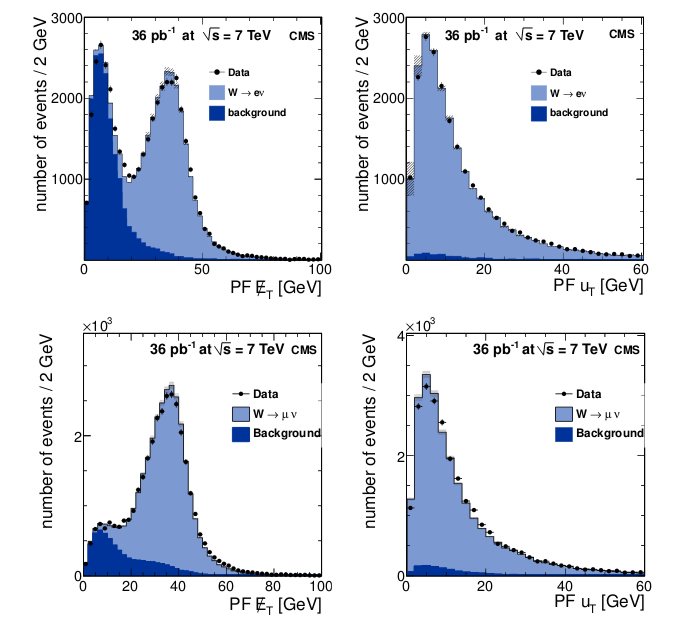
\includegraphics[width=13cm,height=9cm]{/home/tambeebainorbert/Documents/PreOrals/ApprovedPlots2011/MetDistrubution.png}
% \caption{The PF \MET) and $\vert u_{T} \vert$ distribution of  $\displaystyle{ \textsc{W} \rightarrow e\nu}$ (top) and  $\displaystyle{ \textsc{W} \rightarrow \mu\nu}$ 
% (bottom) candidate events. Both data (points) and simulation (solid lines) are shown.}
% \end{figure}
%-Include some detail describtion on how \ETmiss is measured/reconstructed.
%\subsection{Background and signal Monte Carlo}
%\emph{ what constitutes Signal and background and strategies to understand them.}
%\section{Result}
%\subsection{Limits}
%\emph{what to expect as next improvement of work?}
%\section{Excellent Contributions}
\subsection{Current and Future Work}
Our current and future work is directed  in two fronts.
\paragraph{ECAL Timing:}
 Improving on the ECAL timing resolution for mostly high energy photons($\textsc{E} >100$~GeV) remains an important task.
As a good and reliable timing calibration is crucial for background rejection effeciency studies from mostly prompts events from SM model interactions. 
\newline
 We introduce new definition for photon candidate timing such as:
\begin{enumerate}
 \item  Weighted average of \emph{$T_{RECO}$} over the number of channels in cluster; each weight is the error per channel.
 \item  Time of the most energetic reconstructed hit(seed crystal) of the crystal in the cluster.
\end{enumerate}
to improving on the timing measurement.
\paragraph{MET:}
New \MET reconstruction algorithm with variables like \emph{ \MET significance} (\MET \textsc{S})~\cite{MET} could be used to
 quantify the significance in \MET reconstruction by 
evaluating the uncertainty in the total measured transverse momentum, given by 
\begin{equation}
{\displaystyle \vec{\ETmiss}^{total}  \ \ = \ \  - \sum_{i \in X} \vec{\ET}_{i} } 
\end{equation}
where $ \displaystyle {\vec{\ET}_{i}  = (E_{x_{i}},E_{y_{i}})} $  is the measured transverse momentum of the $i^{th}$ reconstructed  object. \text{X} is the
 set of reconstructed objects, such as calorimeter towers (for Calo \MET) or PF particles (for PF \MET ), used to calculate the \MET  .  
A detailed account of this is found in ~\cite{MET}. 
%\emph{Personal Outstanding Issues and Room for Improvements?}
%What  you are going to do next to improve on what has already been done?
\section{Conclusion}
 We have presented a proposal of an analysis to search for GMSB particles using displaced photons  and outlined in detail our candidate strategy for the search.
\newline
 In section 1, we began by introducing GMSB models, stating some of the general and especially theoretical motivations for the choice of these super-symmetry models.
In Section 2, we give a description of
the CMS detector at LHC, stating very important aspects of using this detector in GMSB searches. In section 3,  we outline a possible analysis procedure mentioning 
some of the relevant variables we will consider with detailed description and physics motivated arguments. In the coming years, with improved detector understanding
 and performance, these variables will be very reliable in discriminating background from signal with better efficiency and significance.
% The section ends with brief statements of our current work.
%an outline of our current and future work towards improving on the results obtained by previous groups doing a similar analysis.We conclude in section 4.
% \section{Acknowledgement}
% We want to thank  all our collaborators currently involved in this analysis. We thank Giovanni Franzoni, Seth Cooper, Jared Turkewitz, and Yuichi Kubota for their tremendous work  
% on ECAL timing calibration studies. This has improved on the  ECAL timing measurement of the CMS detector which will continue in the coming years of 
% LHC operation. We want to thank Prof Roger Rusack for providing a unique environment to pursue these studies and for being my co-supervisor. I have learned from him how to be curious
% in the right things and make progress in the right direction.
% All of this would not have been possible without the insight and guidance of Prof Kubota Yuichi. His patience, guidance and hands-on approach has really shaped my understanding
% and interest in experimental Particle Physics.
% Finally, we thank the school of Physics and University of Minnesota for financial support.
\begin{thebibliography}{9}
\bibitem{TIME}CMS Collaboration, ``Time Reconstruction and Performance of the CMS Crystal Electromagnetic Calorimeter``,CFT-09-006, 2009.
\bibitem{KOlive}J.Ellis, J.Hagelin, D. Nanopoulos, K.A. Olive and M. Srednicki; \emph{Nucl. Phys.} B238~(1984) 453; H. Goldberg, \emph{Phys. Rev. Lett} 50~(1983) 1419;
J. Ellis, T. Falk, G. Ganis, K.A. Olive and M. Srednicki, \emph{Phys. Lett.} B 510~(2001) 236, arXiv: hep-ph/0102098.
\bibitem{GMSB}G.F. Giudice and R. Rattazzi ``Theories with Gauge-Mediated Supersymmetry Breaking'' arXiv:hep-ph/9801271v2
\bibitem{g2ex}H. N. Brown et al., Muon $g_{\mu}-2$ Collaboration, \emph{Phys. Rev. Lett} 88~(2002) 2227, hep-ex/0102017; A. Czarnecki and W.J. Marciano,
\emph{ Phys. Rev.} D 64~(2001) 013014, hep-ph/0102122.
\bibitem{g2Theory}M. Knecht and A. Nyffeler, hep-ph/0111058; I. Blokland, A. Czarnecki and K. Melnikov \emph{Phys.Rev. Lett} 88~(2002) 071803 hep-ph/0112117
\bibitem{BSex}CLEO Collaboration, M. S Alan et al., \emph{Phys. Rev. Lett.} 74~(1995) 2885 as updated in S. Amed et al., CLEO CONF 99-10;
BELLE Collaboration hep-ex/0103042
\bibitem{SM}S.Mathin, arXiv:hep-ph/9709356
\bibitem{SUSY}B.Allanach et al,arXiv:hep-ph/0202233v1
\bibitem{LEP}J.Dann et al.(LEPSUSY Working Group), Internal note LEPSUSYWG/97-04(1997), P. Janot, talk at the EPS Conference, Jerusalem, 1997.
\bibitem{CDF}CDF Collaboration, ``Search for Supersymmetry with Gauge-Mediated Breaking in Diphoton Events with Missing Transverse Energy at CDFII ``,\emph{Phys. Rev. Lett.}
\bibitem{ATLAS} ATLAS Collaboration ``Search for Diphoton Events with Large Missing Transverse Momentum in \text{1 $fb^{-1}$} of $\text{7TeV}$ Proton-Proton Collision Data with the ATLAS Detector'', arXiv:1111.4116v1,17th Nov 2011. 
\bibitem{Rome}CMS Draft Analysis,``Search for Long-Lived Particles using Displaced Photons in \emph{PP} Collision at $\sqrt{S}=7TeV$ '', CMS AN AN-11-081 \boldmath{$104(2010) 011801,$}
\bibitem{CMSTDR}CMS Collaboration,``CMS Physics: Technical design report, Volume 1'' CERN-LHCC-2006-001
\bibitem{CORD}CMS uses a right-handed coordinate system, with the origin at the nominal interaction point, the \emph{$x$}-axis pointing to the center of the LHC, 
the \emph{$y$}-axis pointing up (perpendicular to the LHC plane), and the \emph{$z$}-axis along the counterclockwise-beam direction. The polar angle, $\theta$, 
is measured from the positive \emph{$z$}-axis and the azimuthal angle, $\phi$, is measured in the \emph{$x$-$y$} plane. \boldmath{$\displaystyle{\eta = -\ln\tan(\theta/2)}$}. 
The transverse energy and momentum are defined as \boldmath{$\displaystyle{\ET=E\sin\theta}$} and \boldmath{$\displaystyle{\PT=p\sin\theta}$} where \textsc{E} is the energy measured in the 
tracking system.\boldmath{$\displaystyle{\MET = \vert -\sum_{i}\ET^{i}\vec{n_{i}}\vert}$} where $\vec{n_{i}}$ is a unit vector that points from the interaction vertex to the transverse plane.
\bibitem{JINST}CMS Collaboration, ``The CMS experiment at the CERN LHC'', JINST 0803:S08004, 2008.
\bibitem{cmsdata}CMS Collaboration,``CMS trigger and data taking in 2010*'',\boldmath{CMS CR-2011/051}.
\bibitem{RECOAMPLI}CMS Electromagnetic Calorimeter Collaboration, ``Reconstruction of the signal amplitude of the CMS electromagnetic Calorimeter'', Eur.Phys.J.\boldmath{C46S1}(2006)23-35.
\bibitem{Algo} D.del Re et al ``An algorithm for the determination of the flight path of long-lived particles decaying into photons'' CMS AN -2010/212.
\bibitem{PF}CMS Collaboration,``Particle-Flow Event Reconstruction in CMS and Performance for Jets, taus and \ETslash'', CMS Physics Analysis Summary \boldmath{CMS-PAS-PFT-09-001}(2009).
\bibitem{MET2}CMS Collaboration, “Missing Transverse Energy Performance in Minimum-Bias and Jet Events from Proton-Proton Collisions at $\sqrt{s} =7$~TeV ”, CMS Physics Analysis Summary
CMS-PAS-JME-10-004 (2010).
\bibitem{MET}MET JINST (arXiv:1106.5048)
\bibitem{MET}CMS Collaboration, ``Missing transverse energy performance of the CMS detector''; arXiv:1106.5048v1
\bibitem{TDR}CMS Collaboration,``CMS Physics: Technical design report, Volume 2'' CERN-LHCC-2006-001.
\bibitem{ECAL}CMS Electromagnetic Calorimeter Collaboration, ``Energy resolution of the barrel of the CMS Electromagnetic Calorimeter'',JINST 2(2007)P04004.
\bibitem{ECALTDR}CMS Collaboration,``The electromagnetic calorimeter. Technical design report '',. CERN-LHCC-97-33


\end{thebibliography}
\end{document}
